\documentclass[a4paper,12pt,oneside]{book}
\usepackage[utf8]{inputenc}
\usepackage[T1]{polski}
\usepackage{polski}
\usepackage{color}
\usepackage{helvet}
\usepackage{graphicx}
\usepackage{caption}
\usepackage{subcaption}
\usepackage{geometry}
\usepackage{titlesec}
\usepackage{indentfirst}
\usepackage{verbatim}
\usepackage{moreverb}
\usepackage{nameref}
\usepackage{url}
\usepackage{xcolor}
\usepackage[font=footnotesize,labelfont=bf]{caption}
\usepackage{multirow}
\usepackage{booktabs}
\geometry{hmargin={2cm, 2cm}, height=10.0in}
\assignpagestyle{\chapter}{empty}
\newcommand{\param}[1]{\textit{\textless #1\textgreater}}

\DeclareUnicodeCharacter{00A0}{~}

%konfiguracja listingow
\usepackage{listings}
\DeclareCaptionFont{white}{\color{white}}
\DeclareCaptionFormat{listing}{\colorbox{gray}{\parbox{\textwidth}{#1#2#3}}}
\captionsetup[lstlisting]{format=listing,labelfont=white,textfont=white}
\lstset{basicstyle=\footnotesize\ttfamily}
\newcommand{\wykresy}[3] {
	\begin{figure}
		\centering
		\begin{subfigure}[h]{0.3\textwidth}
			\includegraphics[width=\textwidth]{testy/#1_1.png}
			\caption{1 równoległe zapytanie}
		\end{subfigure}
		\begin{subfigure}[h]{0.3\textwidth}
			\includegraphics[width=\textwidth]{testy/#1_2.png}
			\caption{2 równoległe zapytania}
		\end{subfigure}
		\begin{subfigure}[h]{0.3\textwidth}
			\includegraphics[width=\textwidth]{testy/#1_4.png}
			\caption{4 równoległe zapytania}
		\end{subfigure}

		\begin{subfigure}[h]{0.3\textwidth}
			\includegraphics[width=\textwidth]{testy/#1_8.png}
			\caption{8 równoległych zapytań}
		\end{subfigure}
		\begin{subfigure}[h]{0.3\textwidth}
			\includegraphics[width=\textwidth]{testy/#1_16.png}
			\caption{16 równoległych zapytań}
		\end{subfigure}
		\begin{subfigure}[h]{0.3\textwidth}
			\includegraphics[width=\textwidth]{testy/#1_32.png}
			\caption{32 równoległe zapytania}
		\end{subfigure}

		\begin{subfigure}[h]{0.3\textwidth}
			\includegraphics[width=\textwidth]{testy/#1_64.png}
			\caption{64 równoległe zapytania}
		\end{subfigure}
		\begin{subfigure}[h]{0.3\textwidth}
			\includegraphics[width=\textwidth]{testy/#1_128.png}
			\caption{128 równoległe zapytania}
		\end{subfigure}
		\begin{subfigure}[h]{0.3\textwidth}
			\includegraphics[width=\textwidth]{testy/#1_256.png}
			\caption{256 równoległych zapytań}
		\end{subfigure}
		\caption{#2}\label{fig:#3}
	\end{figure}
}


\title{System zautomatyzowanego zarządzania konfiguracją farmy serwerów aplikacji WWW}
\author{Marcin TORGiren Fabrykowski}
\setcounter{secnumdepth}{4}
\setcounter{tocdepth}{4}
\begin{document}
\nocite{*}
%\bibliographystyle{plain}
\bibliographystyle{amsplain}
\thispagestyle{empty}

\includegraphics[height=37.5mm]{agh_nzw_a_pl_1w_wbr_cmyk.eps}\\
\rule{30mm}{0pt}
{\large\textsf{Wydział Fizyki i Informatyki Stosowanej}}\\
\rule{\textwidth}{3pt}\\
\rule[2ex]
{\textwidth}{1pt}\\
\vspace{7ex}
\begin{center}
{\bf\LARGE\textsf{Praca magisterska}}\\
\vspace{13ex}
% --------------------------- IMIE I NAZWISKO -------------------------------
{\bf\Large\textsf{Marcin Fabrykowski}}\\
\vspace{3ex}
{\sf \small kierunek studiów:} {\bf\small\textsf{informatyka stosowana}}\\
{\sf \small specjalność:} {\bf\small\textsf{grafika komputerowa i przetwarzanie obrazów}}\\
\vspace{15ex}
%% ------------------------ TYTUL PRACY --------------------------------------
{\bf\huge\textsf{System zautomatyzowanego zarządzania farmą serwerów aplikacji WWW}}\\
\vspace{14ex}
%% ------------------------ OPIEKUN PRACY ------------------------------------
{\sf \Large Opiekun:} {\bf\Large\textsf{dr inż. Piotr Gronek}}\\
\vspace{22ex}
\textsf{\bf\large\textsf{Kraków, sierpień 2015}}
\end{center}
%% =====  STRONA TYTUŁOWA PRACY INŻYNIERSKIEJ  ====

\newpage

%% =====  TYŁ STRONY TYTUŁOWEJ PRACY INŻYNIERSKIEJ  ====
{\sf Oświadczam, świadomy(-a) odpowiedzialności karnej za poświadczenie nieprawdy, że niniejszą pracę dyplomową wykonałem(-am) osobiście i samodzielnie i nie korzystałem(-am) ze źródeł innych niż wymienione w pracy.}

\vspace{14ex}

\begin{center}
\begin{tabular}{lr}
~~~~~~~~~~~~~~~~~~~~~~~~~~~~~~~~~~~~~~~~~~~~~~~~~~~~~~~~~~~~~~~~~ &
................................................................. \\
~ & {\sf (czytelny podpis)} \\
\end{tabular}
\end{center}

\newpage
\rightline{Kraków, 14 września 2015}
\begin{center}
{\bf Tematyka pracy magisterskiej i praktyki dyplomowej
Marcina Fabrykowskiego.
studenta V roku studiów kierunku informatyka stosowana, specjalności grafika komputerowa i przetwarzanie obarzów.}\\

\end{center}

Temat pracy magisterskiej:
{\bf System zautomatyzowanego zarządzania farmą serwerów aplikacji WWW}\\

\begin{tabular}{rl}

Opiekun pracy:                  & dr inż. Piotr Gronek\\
Recenzenci pracy:               & dr inż. Antoni Dydejczyk\\
Miejsce praktyki dyplomowej:    & Inittec Sp. z o.o., Kraków\\
\end{tabular}

\begin{center}
{\bf Program pracy magisterskiej i praktyki dyplomowej}
\end{center}

\begin{enumerate}
\item Omówienie realizacji pracy magisterskiej z opiekunem.
\item Praktyka dyplomowa:
\begin{itemize}
\item zapoznanie się z rozwiązaniami stosowanymi w dużych środowiskach informatycznych
\item administracja istniejącą infrastrukturą klastrową
\end{itemize}
\item Zapoznanie się z innymi metodami tworzenia klastrów oraz zarządania konfiguracją
\item Testowanie poznanych rozwiązań
\item Ręczne stworzenie klastra WWW oraz sprawdzenie jego działania
\item Opracowanie metody automatycznego konfigurowania maszyn
\item Opracowanie redakcyjne pracy.
\end{enumerate}


\noindent
Termin oddania w dziekanacie: ................\\[1cm]

\begin{center}
\begin{tabular}{lcr}
.............................................................. & ~~~ &
.............................................................. \\
(podpis kierownika katedry) & & (podpis opiekuna) \\
\end{tabular}
\end{center}

\newpage
\linespread{1.3}
\selectfont

\noindent
Na kolejnych dwóch stronach proszę dołączyć kolejno recenzje pracy popełnione przez Opiekuna oraz Recenzenta (wydrukowane z systemu MISIO i podpisane przez odpowiednio Opiekuna i Recenzenta pracy). Papierową wersję pracy (zawierającą podpisane recenzje) proszę złożyć w dziekanacie celem rejestracji.
\newpage
druga recenzja


\vspace{85mm}
\tableofcontents


\addcontentsline{toc}{chapter}{Wstep}
\chapter*{Wstęp}
Niniejsza praca opisuje aplikację ułatwiającą administratorowi tworzenie oraz administrację klasterm dla aplikacji WWW.\\
Została ona podzielona na pięć rozdziałów tworzących trzy grupy.\\
Pierwsza grupa skupia się na rozważaniach teoretycznych.
W jej skład wchodzą rozdziały:
\begin{description}
\item{"Wstęp do klastrowania"}\\
Opisuje on powody z których zaczęto stosować klastry WWW.
Przybliża podział klastrów oraz cechy każdego rodzaju.
Dodatkowo zarysowywuje problem wynikający z trudności zarządzania konfiguracją na klastrach.
\item{"Metody klastrowania"}
Rozdział ten opisuje najbardziej znane metody służące klastrowaniu aplikacji.
Opisuje on metody takie jak \textit{DNS round robin}, \textit{Nginx upstream}, \textit{Haproxy}, \textit{LSV}.
Każda z powyższych metod zostałą krótko opisana, sposób jej działania oraz sposób konfiguracji.
\item{"Zarządzanie konfiguracja"}\\
Ten rozdział przedstawia problem konsystentnej konfiguracji dużej ilości serwerów.
Opisuje on podstawowy, ręczny sposób konfiguracji maszyn.
Jego zalety i wady, a następnie kolejne metody usprawniające i eliminujące wady ręcznej konfiguracji.
Zostały opisane aplikacje takie jak: \textit{Fabric}, \textit{Puppet}, \textit{CFEngine}, \textit{Ansible}, ze szczególnym naciskiem na ostatni.
\end{description}

W drugiej części pracy, znajduje się jeden rozdział, opisujący praktyczne testy wydajnościowe opisywanych wcześniej metod klastrowania.
Skupia się on zarówno na testowaniu możliwości zwiększania wydajności jak i zapewnianiu wysokiej dostępności.

Trzecia część opisuje tytułowy \textit{System zautomatyzowanego zarządzania konfiguracją farmy serwerów aplikacji WWW}.
Opisuje on powody wyboru konkretnych technologii, opis ich konfiguracji oraz sposobu współdziałania.

\chapter{Wstęp do klastrowania}
\label{ch:wstep_do_klastrowania}
\section{Idea klastrowania}
W czasach kiedy powstał internet, narodziła się potrzeba udostępniania informacji. Początkowo był to zwykle czysty tekst, który umieszczano na wtedy standardowych komputerach. Liczba odbiorców również nie była nie była duża, co wynikało z dopiero tworzącej się sieci internet.
W miarę upływu czasu, strony internetowe zaczęły się rozrastać. Zaczęto dodawać obrazy a następnie animacje i inne elementy poprawiające możliwości stron oraz odczucia wizualne. Zaczęła również, w związku z coraz łatwiejszym dostępem do internetu, liczba użytkowników chcących uzyskać dostęp do stron.\\
Wymusiło to potrzebę używania coraz to mocniejszych maszyn do serwowania treści. Niestety, liczba użytkowników oraz wymagań stawianych stronom internetowym rosła szybciej niż postępował rozwój mocy obliczeniowych komputerów. Zaczęto używać dedykowanych serwerów dla aplikacji WWW zamiast zwykłych komputerów domowych. Jednak i to okazało się niewystarczające w obliczu wymaganiom stawianym przez dzisiejszy świat.

Aby rozwiązać ten problem, narodziła się idea połączenia kilku maszyn w jeden twór, tak aby zwiększyć całkowitą moc przeznaczoną na serwowanie treści.
\section{Rodzaje klastrów}
Istnieją dwa główne rodzaje klastrów.
\begin{itemize}
\item klastry wysokiej dostępności
\item klastry wysokiej wydajności
\end{itemize}ch 
Podział ten nie jest jednak bardzo sztywny.
Niektóre rzeczywiste klastry należą tylko do jednej grupy, jednak najczęściej mają one cechy obu tych grup.
\subsection{Klastry wysokiej dostępności}
Klastry wysokiej dostępności (ang. \textit{high availability, HA}) tworzone są głównie po to, aby zapewnić jak najwyższy poziom dostępności danej usługi.
Konstrukcje te składają się zwykle z wielu maszyn, z których jakaś część nie uczestniczy w serwowaniu danych, a jedynie czeka w gotowości i w przypadku awarii maszyn aktywnych, przejmuje ich zadanie. Efektem jest ciągła dostępność usługi dla klienta.\\
Brak dostępności portalu może wiązać się z kosztami bądź brakiem zysków dla właściciela, dlatego często stosuje się klastry wysokiej dostępności.
\subsection{Klastry wysokiej wydajności}
Klastry wysokiej wydajności (ang. \textit{high performance, HP}) tworzone są głównie po to, aby zapewnić jak najwyższy poziom wydajności danej usługi.
Celem tego typu klastrów jest zapewnienie komfortu korzystania z serwisu dla klienta. W tej architekturze, pracują wszystkie maszyny, oraz każda z nim wykonuje jakąś część zadania w celu jak najszybszego skonstruowania odpowiedzi dla klienta.\\
W wersji ideowej, awaria jakiejś maszyny, unieruchamia klaster, ponieważ nie jest możliwe uzyskanie części odpowiedzi za którą odpowiadała maszyna która uległa awarii. W praktyce rzadko spotyka się czyste klastry wysokiej wydajności.
\subsection{Klastry mieszane}
Klastry mieszane są najczęściej spotykanymi klastrami. Posiadają one cechy obu powyższych grup, czyli najczęściej pracują wszystkie maszyny w klastrze, jednak ich konfiguracja pozwala im na wykonywanie dowolnego zadania (z puli przewidzianych zadań), w taki sposób, że podczas pracy wszystkich maszyn w klastrze, następuje szybsza odpowiedź do klienta - cecha wysokiej wydajności - jednak po awarii którejś z maszyn, pozostałe są w stanie przejąć jej obowiązki pozwalając odpowiedzieć na zapytanie - wysoka dostępność.\\
Można zauważyć, że podczas awarii węzłów w takim rodzaju klastra, spada wydajność, lecz zachowana jest ciągłość dostępu usługi, bo zwykle daje czas administratorowi na usunięcie usterki, bądź - jak zostanie pokazane w dalszej części tej pracy - skonfigurowanie nowych węzłów w celu zastąpienia tych które uległy awarii.
\section{Zarządzanie konfiguracją}
W czasach gdy strony były serwowane przez ich twórców na ich własnych komputerach, oni sami dbali o konfigurację swojej maszyny aby spełniała swoje zadanie.\\
W miarę jak zaczęto potrzebować coraz to większych mocy obliczeniowych, zaczęto wynajmować mocne serwery z dobrymi łączami, aby to one serwowały dane dla klientów.
Konfiguracją takiego serwera zajmował się twórca strony, bądź zatrudniony administrator.

Jednak, gdy zaczęto używać klastrów pojawił się problem ich konfiguracji. Gdy klaster składał się z kilku węzłów, było bardzo mozolną pracą skonfigurowanie każdego węzła osobno oraz pilnowanie, aby konfiguracje na każdym węźle były odpowiednie.
Po przypadkowej zmianie parametrów konfiguracji na jednej maszynie, trudno jest później znaleźć błąd.

Problem pojawił się również, gdy klastry zaczęły mieć więcej niż kilka węzłów. Skonfigurowanie kilkuset maszyn nie było prostym zadaniem, jak również prowadziło do wielu pomyłek. Dlatego administratorzy klastrów starali się ułatwić sobie pracę a zarazem uniknąć przypadkowych błędów.\\
Tak też powstały narzędzia do kontrolowania konfiguracji na wielu maszynach.

\chapter{Metody klastrowania}
W rozdziale tym przedstawię podstawowe metody wykorzystywane przy tworzeniu klastrów pod aplikacje internetowe.
\section{DNS round robin}
\subsection{Czym jest DNS}
DNS (ang {\textit{Domain Name System}) jest to system nazw domenowych. Usługa której najważniejszą funkcją jest przyporządkowanie nazwom domenowym (czytelnym dla człowieka) adresów IP.
Oznacza to, że system taki, jest w stanie zamienić nazwę \texttt{www.ftj.agh.edu.pl} na adres \texttt{149.156.110.3}.
Funkcjonalność taka w znacznym stopniu ułatwia korzystanie z sieci Internet, ponieważ przeciętnemu człowiekowi jest prościej zapamiętać mnemonik \texttt{www.ftj.agh.edu.pl} bądź \texttt{www.duckduckgo.com} niż ciągi czterech liczb.
Do zamiany nazwy domenowej na adres IP służą rekordy \texttt{A} oraz \texttt{AAAA}, wykorzystywane odpowiednio do adresów IPv4 oraz IPv6.
Przykład zastosowania rekordu \texttt{A} przedstawiam na poniższym listingu:
\lstinputlisting{lst/rr_arecord.lst}
w powyżej konfiguracji widzimy, że odpytując server DNS o wartość \texttt{nazwa4.domenowa.pl} otrzymamy informację, że dana nazwa wskazuje na adres \texttt{1.2.3.4}.\\
Innymi, często spotykanymi rekordami są rekordy \texttt{CNAME}, \texttt{MX} oraz \texttt{TXT}.
\begin{description}
\item[CNAME] jest to rekord będący wskaźnikiem. Dla przykładu:
\lstinputlisting{lst/rr_cname.lst}
widzimy, że w powyższym przykładzie \texttt{nazwa.domenowa.pl} wskazuje na 1.2.3.4.
Chcąc aby, \texttt{www.nazwa.domenowa.pl} również wskazywała w to samo miejsce, moglibyśmy również zdefiniować ją jako rekord \texttt{A} z takim samym adresem.
Jednak, w przypadku migracji serwera z adresu \texttt{1.2.3.4} na \texttt{1.2.3.5}, należałoby zmieniać ten adres w obu rekordach.
Zastosowanie rekordu \texttt{CNAME}, pozwala powiedzieć "nazwa \texttt{www.nazwa.domenowa.pl} wskazuje w to samo miejsce, w które wskazuje \texttt{nazwa.domenowa.pl}".
Prowadzi to do zmniejszenia ryzyka pomyłki przy wpisywaniu adresów IP, jak również zmniejsza liczbę miejsc w których należy zmienić adresację w przypadku migracji serwera.
\item[MX] rekord wskazujący na adres serwera pocztowego obsługującego daną domenę.
Strefa może zawierać kilka rekordów \texttt{MX} w celu dystrybucji ruchu na kilka serwerów pocztowych.
\lstinputlisting{lst/rr_mxrecord.lst}
Widzimy, że wpis definiujący rekord \texttt{MX} nie posiada nazwy. Zwykle rekord ten definiowany jest na początku definicji strefy, dlatego pominięcie nazwy powoduje, ze rekord ten odnosi się do nazwy tej strefy.
Jest to kolejna rzecz które uogólnia konfigurację i ułatwia migrowanie.
Wartość \texttt{5} oznacza poziom preferencji danego serwera. Mając zdefiniowanych kilka rekordów \texttt{MX}, poczta jest dystrybuowana przy pomocy algorytmu ważonego round robin.
\item[TXT] rekord który zgodnie z założeniami DNS miał zawierać dane tekstowe czytelne dla człowieka.
Obecnie rzadko zawiera dane dla użytkowników. Wykorzystywany jest głównie do konfiguracji SPF, co wykracza poza tematykę tej pracy.
\end{description}
\subsection{Opis metody}
Metoda ta polega na odpowiednim skonfigurowaniu strefy na serwerze DNS, w taki sposób, aby pod jedna nazwa rozwiązywała się na kilka adresów IP.
W efekcie, gdy serwer otrzyma zapytanie o daną nazwę domenową, zostanie mu zwrócona pula adresów zamiast jednego.
Aplikacja która otrzyma listę adresów IP, powinna połączyć się na losowy z nich.
Niestety nigdy nie ma pewności, że aplikacja posiada zaimplementowaną obsługę wielu adresów zwracanych przez serwer DNS, dlatego serwer wprowadza zabezpieczenie przed takim zachowaniem, a mianowicie tytułowy algorytm \textit{round robin}, który zwraca adresy IP, jednak za każdym razem ich permutację.\\
Dla przykładu, poniżej zamieszczone trzy zapytania wykonane po sobie.
\lstinputlisting{lst/rr_dig.shell}
Widzimy, że przy każdym zapytaniu, jako pierwszy adres zwracany jest kolejny adres z puli. Zapewnia to prawidłowe balansowanie ruchu, nawet przy aplikacjach nie potrafiących obsłużyć wielu adresów i łączących się na pierwszy otrzymany.

Metoda ta jest metodą wysokiej wydajności, ponieważ pozwala w sposób niewidoczny dla użytkownika rozdzielić ruch na kilka serwerów, a tym samym rozłożyć obciążenie, to skutkować będzie szybszą odpowiedzią klientowi na zapytanie.
Metoda ta nie zapewnia natywnie wykrywania niedostępności któregoś z serwerów, dlatego nie może służyć bezpośrednio jako metoda wysokiej dostępności.
Pośrednio występuje tutaj jednak mechanizm broniący przed niedostępnością któregoś z serwerów. W przypadku gdy aplikacja próbować się będzie połączyć z losowym adresem z puli, a połączenie nie będzie mogło być nawiązane, osiągnięty zostanie limit czasu połączenia (tzw. \textit{timeout}. W takiej sytuacji, dobrze napisana aplikacja, będzie próbować połączyć się na kolejny adres z puli, w nadziei, że będzie on dostępny.
W takiej sytuacji, połączenie zostanie nawiązane i klient otrzyma odpowiedź, jednak do czasu generowania odpowiedzi, trzeba doliczyć czas potrzebny na osiągnięcie \textit{timeout-u}. Może on wynieść od kilku, do kilkudziesięciu sekund.

Metoda ta jest również zależna od działania serwera DNS.
Najprostszym sposobem ochrony przed awarią tego systemu dystrybucji ruchu jest skonfigurowanie \textit{Secondary DNS}. To jednak wykracza poza tematykę tej pracy.
\subsection{Konfiguracja}
Konfiguracja DNS round robin jest stosunkowo prosta.
W konfiguracji strefy, należy umieścić wpis z wieloma rekordami \textit{A} dla jednej nazwy.
Przykład takiej strefy zamieszczony został poniżej
\lstinputlisting[caption=mgr.fabrykowski.pl.zone]{lst/rr_zone.zone}
W powyższym przykładzie, dla nazwy \texttt{rr.mgr.fabrykowski.pl} zostały zdefiniowane trzy adresy IP.
\section{Nginx}
\subsection{Czym jest nginx}
Nginx jest serwerem proxy oraz serwerem treści statycznych.
Wykorzystywany jest zwykle w połączeniu z serwerem Apache który serwuje treści PHP, podczas gdy sam dostarcza pliki statyczne (JavaScript, CSS, JPEG itp).
Drugim często wykorzystywanym modelem wykorzystania Nginx-a jest serwowanie treści statycznych oraz wykonywanie \textit{fastcgi pass}
\paragraph{Fastcgi pass} \hspace{0pt} \\
Moduł ten pozwala na komunikacje z procesami FastCGI.
Wykorzystanie FastCGI daje dużą niezależność w technologi opracowania aplikacji, która może zostać wykonana w PHP, Pythonie bądź Rubym.
Istnieje również możliwość zmiany wersji aplikacji, bądź technologii jej wykonania bez zmian w konfiguracji serwera, jeżeli aplikacja udostępnia to samo api FastCGI.

Do obsługi języka PHP zostanie wykorzystany php-fpm (\textit{PHP FastCGI Process Manager}.
Jest to alternatywna implementacja PHP FastCGI.
Pozwala ona na większą kontrolę w zakresie pul procesów - ich liczby oraz sposobu uruchamiania, jak również dowolność w kwestiach sieciowych - adres oraz port do nasłuchiwania.

Porównanie testów wydajności PHP-fpm oraz mod\_php do Apache jak również szybkość serwowania treści statycznych zostanie przedstawione w późniejszych rozdziałach.
\subsection{Opis metody}
Metoda klastrowania przy pomocy Nginx-a polega na zdefiniowaniu sekcji \texttt{upstream}.
Pozwala to na skonfigurowanie puli adresów do których będą przekazywane zapytania.
Aby dodać serwer do puli, należy podać jego adres IP bądź nazwę domenową oraz port.

Zapytania do serwerów wykonujących (\textit{workerów}) rozdzielane są równomiernie pomiędzy wszystkie serwery w puli.\\
Pozwala to na obsługiwanie zapytań na wielu maszynach, dlatego metoda ta pozwala na tworzenie klastrów \textbf{wysokiej wydajności}.

Ponadto, zaimplementowany jest również mechanizm sprawdzający stan poszczególnych serwerów w puli i w przypadku wykrycia awarii, oznaczany jest on jaki \textit{failure} i zapytanie nie są do niego kierowane.\\
Jest to zachowanie typowe dla klastrów \textbf{wysokiej dostępności}

Istnieje możliwość modyfikacji domyślnego algorytmu używanego przez Nginx-a.
\begin{itemize}
	\item zmiana sposobu dystrybucji zapytań dodając opcjonalny parametr \texttt{weight} mówiący o wadze danego węzła. Dla przykładu, w poniższej konfiguracji:
	\lstinputlisting{lst/nx_weight.conf}
	na każde 6 zapytań do \texttt{pula1}, 5 zostanie przekazanych do \texttt{server1} a jedno do \texttt{server2}.
	Opcja ta wykorzystywana jest głównie tam, gdzie poszczególne serwery różnią się parametrami bądź obciążeniem nie wynikającym z obsługiwania tej puli.
	\item zmiana sposobu określania serwera jako niedostępnego.
	Służą do tego parametry \texttt{max\_fails}, \texttt{fail\_timeout} oraz \texttt{slow\_start}.\\
	\begin{description}
	\item[\texttt{max\_fails}] określa liczbę nieudanych prób komunikacji z serwerem w czasie \texttt{fail\_timeout} nim serwer zostanie oznaczony jako niedostępny.
	Domyślna wartość tego parametru wynosi 1, natomiast wartość 0 wyłącza oznaczanie serwerów jako niedostępne.
	\item[\texttt{fail\_timeout}] określa czas w jakim musi nastąpić \texttt{max\_fails} nim serwer zostanie uznany za niedostępny.
	Określa również interwał czasowy co który będzie sprawdzana dostępność serwera.
	Wartość domyślna dla tego parametru wynosi 10 sekund.
	\item[\texttt{slow\_start}] określa czas w jakim będzie zwiększana wartość \texttt{weight} od zera do docelowej po przejściu serwera ze stanu niedostępnego do stanu dostępnego.
	Wartość domyślna wynosi 0, co oznacza wyłączone płynne włączanie serwera do puli.
	\end{description}
	\item oznaczenie konkretnych serwerów, jako serwerwy zapasowe.  
	Powoduje to nieprzekazywanie zapytań do tych serwerów jeżeli wszystkie serwery podstawowe odpowiadają.
	W przypadku, gdy któryś z podstawowych serwerów zostanie oznaczony jako niedostępny, zapytania zostają przekazywane do któregoś z serwerów zapasowych.
	Powoduje to zachowanie \textbf{wysokiej wydajności} oraz \textbf{wyskokiej dostępności}.	
\end{itemize}
\subsection{Konfiguracja}
TODO
\section{Haproxy}
\subsection{Czym jest haproxy}
\subsection{Konfiguracja}
\section{LVS}
TODO

\chapter{Zarządzanie konfiguracją}
W rozdziale tym przedstawię różne metody zarządzania konfiguracją serwerów. Postaram się opisać poglądowo różne metody, jak również przedstawić zalety i wady poszczególnych z nim.
\section{Ręczna konfiguracja każdego serwera za pomocą SSH}
\subsection{Opis}
Ręczna konfiguracja serwerów stos osuwana jest głównie tam, gdzie administrator ma pod swoją opieką jeden bądź kilka serwerów. W takim przypadku zmiana konfiguracji na serwerze jest prosta i nie zajmuje dużej ilości czasu.\\
Konfiguracja taka nie wymaga od administratora żadnej wiedzy wykraczającej poza obszar konfigurowanego systemu oraz usług, a wprowadzane zmiany widoczne są od razu po wprowadzeniu.
Ten sposób konfiguracji spotykany jest czasem w większych systemach informatycznych.
Dzieje się tak zwykle w jednostkach szybko rozwijających się, gdzie nastąpił szybki wzrost liczby serwerów i nie opracowano jeszcze metoda automatyzacji konfiguracji.

Do konfiguracji ręcznej nie potrzeba żadnego dodatkowego oprogramowania ani po stronie maszyn konfigurowanych, ani maszyny z której następuje konfiguracja.
Na maszynie z której następuje konfiguracja musi być dostępny klient SSH, który jest instalowany domyślnie we wszystkich dystrybucjach systemów GNU/Linux, a na maszynach konfigurowanych musi być zainstalowany i uruchomiony serwer SSH - jest on domyślnie zainstalowany w większości dystrybucji serwerowych GNU/Linux i w części dystrybucji przeznaczonych na komputery domowe.

Wadą takiej metody jest również sytuacja, w której tylko jedna osoba, bądź mała grupa osób, zna konfigurację poszczególnych serwerów oraz usług.
W przypadku opuszczenia przez daną osobę zespołu, pozostali członkowie muszą, analizując pliki konfiguracyjne, zrozumieć zamysł osoby to tworzącej.\\
Kolejną wadą, jest brak możliwości powielenia konfiguracji.
W przypadku gdy zaistnieje potrzeba skonfigurowania bliźniaczego serwera, jako serwera zapasowego, należy każdą usługę skonfigurować od nowa na wzór serwera pierwotnego. Również wprowadzane zmiany należy uwzględniać na wszystkich serwerach.
Może to w prosty sposób prowadzić do błędów i rozbieżności konfiguracji.
\subsection{Zalety i wady}
Zalety:
\begin{itemize}
\item prostota
\item używanie tylko domyślnych komponentów systemu
\item szybkość wprowadzanych zmian
\item informacja zwrotna czy usługa została uruchomiona poprawnie
\end{itemize}
Wady:
\begin{itemize}
\item \textbf{brak skalowalności}
\item różnice między poszczególnymi serwerami
\item trudność powielania
\item wiedza o konfiguracji zależna od jednego pracownika
\end{itemize}
\subsection{Przykład}
\lstinputlisting{lst/conf_ssh.sh}
\subsection{CSSH}
Istnieje narzędzie CSSH (\textit{Cluster SSH}) które wychodzi na przeciw osobą chcącym konfigurować kilka serwerów jednocześnie poprzez SSH.
Narzędzie to potrafi otworzyć wiele sesji SSH równolegle - każda sesja w osobnym terminalu.
Głównym interface-em programu, jest małe okno wejścia, które przechwytując wpisywany do niego tekst, przesyła go do wszystkich otwartych sesji.\\
Zmniejsza to prawdopodobieństwo rozbieżności w konfiguracji, jak również przyśpiesza proces, ponieważ tekst jest wpisywany do wszystkich sesji jednocześnie i nie ma potrzeby wielokrotnego wpisywania tej samej konfiguracji na wielu maszynach.\\
Aplikacja umożliwia również przełączenie się w dowolnej chwili na konkretny terminal i interakcję tylko z jednym serwerem, np: w celu zdiagnozowania problemu występującego tylko na tej jednej maszynie.
\section{Fabric}
\subsection{Opis}
Jest aplikacją napisaną w języku Python, służącą głównie do wykonywania poleceń powłoki na zdalnym serwerze. Aplikacja pozwala na zdefiniowanie kolejności w jakiej mają zostać poszczególne polecenia, jak również udostępnia kilka funkcji sprawdzających, np: czy plik istnieje, bądź kopiowanie plików na lub z serwera.\\
Sprawdza się wszędzie tam, gdzie chcemy wykonać konkretne operacje na zdalnym systemie niezależnie od aktualnego stanu tego systemu, bądź z niewielkim wpływem obecnych czynników.
Zastosowanie fabrica można porównać do CSSH, z tą różnicą, że operacje nie są wpisywane przez administratora podczas sesji, a zdefiniowane wcześniej w pliku, co w znacznym stopniu ułatwia powtarzalność wykonywania zdefiniowanych operacji.
Pozwala również w prosty sposób rozdzielić zdefiniowane zadania na poszczególne grupy serwerów na których należy je wykonać.\\
Typowe zastosowania:
\begin{itemize}
\item restart nietypowych usług nie posiadających jeszcze odpowiednich skryptów sysvinit
\item rekonfiguracja projektów na zdalnych serwerach po wysłaniu zmian przez system kontroli wersji
\item przeszukiwanie logów poszczególnych serwerów
\end{itemize}
\subsection{Zalety i wady}
Zalety:
\begin{itemize}
\item łatwość instalacji - repozytoria dystrybucji oraz pythonowe
\item równoległe wykonywanie operacji
\item łatwość konfiguracji
\item powtarzalność wykonywania
\item skalowalność
\item niewymagana instalacja oprogramowania na zdalnych maszynach
\end{itemize}
Wady:
\begin{itemize}
\item ograniczone możliwości decyzji na podstawie aktualnej konfiguracji
\item wykonywanie tylko poleceń powłoki
\end{itemize}
\subsection{Przykład}
\lstinputlisting[language=python,caption=fabfile.py]{lst/conf_fabfile.py}
przykład działania powyższego skryptu:
\lstinputlisting{lst/conf_fabfile_run.sh}
Aplikacja została uruchomiona z parametrami:
\begin{description}
\item[-P] równolegle wykonywanie zadań
\item[-z 5] uruchomienie pięciu równoległych połączeń
\item[-I] zapytanie o hasło do serwerów (używane gdy niedostępne logowanie po kluczach SSH)
\item[show\_problem] nazwa zadania zdefiniowana w pliku \texttt{fabfile.py}
\end{description}
Fabric wykonuje połączenia do hostów zdefiniowanych w zmiennej \texttt{env.hosts} w liczbie pięciu połączeń równoległych.
W przypadku nie podania parametru \texttt{-z}, aplikacja wykona liczbę równoległych połączeń równą liczbie zdefiniowanych hostów dla danego zadania.\\
Po połączeniu się do zdalnego hosta, następuje sprawdzenie czy istnieje plik \texttt{/var/problem}. W przypadku wykrycia istnienia takiego pliku, zostaje wywołane polecenie powłoki \texttt{cat}.
W wyniku wykonywania widzimy, ze plik \texttt{/var/problem} istniał tylko na serwerze o adresie IP \texttt{192.168.0.12} i zawierał tekst \textit{zasob byl podmontowany}.
\section{Puppet}
\subsection{Opis}
\label{sec:puppet_opis}
Puppet jest jednym z najbardziej rozpowszechnionych systemów do zarządzania konfiguracją.
U podstaw ideologii działania puppeta stoi definicja oczekiwanego stanu serwera.
Administrator definiuje oczekiwany stan systemu, np: istnienie użytkownika o podanych parametrach, bądź istnienie pliku o zadanej zawartości, a puppet dąży do uzyskania takiego stanu - stworzy użytkownika lub plik taki aby spełniał zadane wymagania.\\
Puppet został napisany w języku Ruby, co wpływa na składnię manifestów przez niego wykorzystywanych.
Manifest jest opisem żądanego stanu danego obiektu (użytkownik, plik, zamontowany zasób).
Manifesty są zapisywane w plikach \texttt{*.pp}.\\
Puppet działa w trybie klient-serwer.
Serwer posiada zapisane manifesty dla wszystkich maszyn, dlatego w celu rekonfiguracji wielu maszyn, wystarczy zmiana jedynie w centralnym punkcie - serwerze \textit{master}.\\
Istnieją trzy możliwości wykonywania manifestów.
\begin{description}
	\item{bezpośrednio na maszynie}
		poprzez jawne wywołanie manifestu na danej maszynie, następuje jego sparsowanie oraz zastosowanie zawartych w nim deklaracji do lokalnej maszyny
	\item{cykliczne pobieranie danych przez agenta}
		ponieważ puppet w zamyśle ma działać w trybie \textit{pull}, dlatego jest to jego domyślny tryb pracy.
		Agent, działający na maszynach klienckich - maszynach których stan ma być kontrolowany przez puppeta - w cyklicznych odstępach czasu pobiera z serwera \textit{master} żądaną konfiguracje.
		Nie pobiera on bezpośrednio manifestów zapisanych przed administratora, lecz skompilowaną ich wersję specjalne dla tej maszyny.\\
		Połączenia do \textit{master}-a są szyfrowane poprzez SSL co zwiększa bezpieczeństwo przesyłanych danych wrażliwych zawartych w manifestach.
	\item{wymuszone uruchomienie agenta}
		tryb ten działa podobnie do cyklicznego pobierania danych, z tą różnicą, ze użytkownik jawnie zmusza agenta do poprania danych z serwera \textit{master} natychmiast, zamiast czekać aż agent pobierze te dane samoistnie.
\end{description}
\subsection{Zalety i wady}
Zalety:
\begin{itemize}
	\item popularność
	\item duże zaplecze \textit{community}
	\item dojrzałość projektu
\end{itemize}
Wady:
\begin{itemize}
	\item potrzeba instalacji oprogramowania na maszynach klienckich
	\item działanie w trybie \textit{pull}
	\item skomplikowana instalacja
\end{itemize}

\section{CFEngine}
\subsection{Opis}
CFEngine jest jednym z najstarszych systemów do zarządzania konfiguracją.
Powstał z myślą o systemach w których nie jest zapewniona dostateczna jakoś łącza, np: łodzie podwodne.

Z racji swojego wieku, architektura CFEngine, w odpowiedzi na zmieniające się potrzeby systemów, ulegała zmianom.
Aktualnie rozwijana jest trzecia generacja CFEngine.
Kolejne generacje starały się upraszczać składnie konfiguracji oraz zwiększać możliwości oferowane przez oprogramowanie.

CFEngine opiera się na "Teorii obietnic".
Jest to teoria stojąca u podstaw wszystkich systemów zarządzania konfiguracją. W celu opisu teorii obietnic por. z \ref{sec:puppet_opis}.

CFEngine, podobnie jak Puppet działa w trybie \textit{pull}, czyli agent pobiera dane z centralnego serwera.
W przeciwieństwie do Puppeta, CFEngine zapisuje pobrane \textit{polityki} na lokalnej maszynie, dzięki czemu w przypadku braku łącza do maszyny centralnej, jest w stanie kontrolować i ewentualnie korygować konfigurację maszyny w stanie offline.
\subsection{Zalety i Wady}
Zalety:
\begin{itemize}
	\item dojrzałość projektu
	\item odporność na przerwy w działaniu łącza
	\item bardzo duża skalowalność
\end{itemize}
Wady:
\begin{itemize}
	\item trudna konfiguracja
	\item trudna instalacja
\end{itemize}
\section{Ansible}
\subsection{Opis}
Ansible jest również narzędziem do zarządzania konfiguracja serwerów. Został napisany w języku Python i w przeciwieństwie do poprzedników nie wymaga instalacji żadnego oprogramowania na maszynach klienckich.
Wymaga jedynie, aby na maszynach które będą miały być obsługiwane przez Ansible, był zainstalowany serwer SSH oraz interpreter języka Python. Obie te rzeczy są instalowany domyślnie przez znaczna większość dystrybucji.
Zalecane jest również skonfigurowanie logowania przy użyciu kluczy SSH, jednak wpływa to tylko na bezpieczeństwo i wygodę użytkowania.\\
\subsubsection{Tryb aktywny i pasywny}
Inną cechą odróżniającą Ansible od jego alternatyw jest kierunek działania.
Ansible jest system działającym w trybie aktywnym, natomiast Puppet, Chef bądź CFEngine działają pasywnie.
Znaczy to, że działanie Ansible jest wymuszane przez administratora poprzez wywołanie odpowiedniego \textit{playbooka}, w przeciwieństwie do pozostałych, gdzie demon działający na serwerze klienckim odpytuje serwer z konfiguracją w celu pobrania aktualnych polityk.
Ansible tutaj daje administratorowi większe pole do działania, ponieważ, po wykonaniu \textit{playbook}-a dostaje on raport, jakie kroki zostały podjęte, które polityki były spełnione a które nie, oraz czy jakieś akcje się nie powiodły.\\
Pozwala on również w prosty sposób na konfigurację działania w trybie quasi-pasywnym poprzez zastosowanie np: \textit{cron}-a do cyklicznego wykonywania \textit{playbook}-a.
W efekcie Ansible daje możliwość pracy w trybie aktywnym jak i pasywnym.
\subsubsection{Instalacja}
Istnieje kilka metod instalacji Ansible
\begin{itemize}
\item ze źródeł\\
Jest to najprostsza metoda instalacji. Ponieważ Ansible jest napisane w języku Python, nie wymaga on kompilacji ani ingerencji w system.
\lstinputlisting{lst/ansible_install_git.sh}
Metoda ta wymaga jednak aby w systemie zainstalowane były biblioteki Pythonowe:
\begin{itemize}
\item paramiko
\item PyYAML
\item jinja2
\item httplib2
\end{itemize}
Wykonanie powyższego kodu powoduje przełączenie się na wirtualne środowisko Pythona przygotowane przez developerów Ansible.\\
Wirtualne środowisko zostanie opisane w kolejnym podrozdziale.
\item przez repozytorium\\
Ansible jest obecne w repozytorium praktycznie każdej dystrybucji. Instalacja zależna jest od konkretnej dystrybucji.\\
Ta metoda może powodować problemy z używaniem Ansible w wirtualnym środowisku Pythona ponieważ narzędzie instalowane jest globalnie, natomiast środowisko wirtualne często tworzone jest bez dostępu do globalnych bibliotek.
\item przez PIP\\
Jest to zalecana metoda instalacji, ponieważ łączy w sobie prostotę procesu z elastycznością.
Wykorzystuje on repozytorium bibliotek Pythonowych - \texttt{pip}.\\
Instalacja Ansible poprzez \texttt{pip} wymaga wykonania polecenia:\\
\lstinputlisting{lst/ansible_install_pip.sh}
spowoduje ono ściągnięcie najnowszej wersji Ansible jak również zależnych pakietów.
Instalacja odbędzie się do katalogów zdefiniowanych w zmiennych środowiskowych. Domyślnie są do główne katalogi \texttt{/usr} jednak mogą one zostać nadpisane przez użycie wirtualnego środowiska.
\end{itemize}
\subsubsection{Wirtualne środowisko Pythonowe}
Wirtualne środowisko jest narzędziem pozwalającym na stworzenie odizolowanego od bibliotek systemowych środowiska uruchomieniowego dla aplikacji pythonowych.\\
Nowe środowisko tworzone jest przy pomocy polecenia \texttt{virtualenv}.
Tworzy ono strukturę katalogów potrzebną interpreterowi Pythona do działania. Poniżej znajduje się przykład takiej struktury:
\lstinputlisting{lst/ansible_install_tree.sh}
Poleceniem \texttt{source <plik\_aktywacji>} aktywujemy wirtualne środowisko.
Powoduje to nadpisanie domyślnych ścieżek przeszukiwania z domyślnych systemowych na lokalne w wirtualnym środowisku.
Następnie należy uruchamiać interpreter Pythona nie podając bezpośredniej ścieżki do niego (np: \texttt{/usr/bin/python2}) lecz poprzez zmodyfikowane środowisko: \texttt{/usr/bin/env python}.
Całość pozwala na tworzenie wirtualnych środowisk ze specyficznymi wersjami Pythona, różnymi niż domyślny interpreter w systemie jak również instalacja odpowiednich bibliotek dla konkretnego projektu a nie dla całego systemu.
Używanie wirtualnego środowiska nie wymaga również posiadania konta administratora.  
Wirtualne środowisko zwiększa również przenośność projektów.
Istnieje możliwość wyeksportowania do pliku tekstowego przy pomocy \texttt{PIP}-a listy zainstalowanych wraz z ich wersjami.
Pozwala on również za zaimportowanie na nowym środowisku, dokładnie tych samych bibliotek, to tworzy dokładną kopię środowiska źródłowego oraz ułatwia migrację aplikacji pomiędzy maszynami.
\subsection{Struktura}
Struktura Ansible jest bardzo prosta i skupia się na trzech podstawowych elementach. Są nimi:
\begin{description}
\item {inventory}\\jest to plik zawierający listę hostów które mają być zarządzane.
\item {moduły}\\Ansible używa modułów w celu wykonywania konkretnych operacji. Pozwala na pisanie własnych modułów.
\item {playbooki}\\pliki zawierające całościowy opis stanu jaki ma zostać osiągnięty na konfigurowanych hostach.
\end{description}
\subsubsection{Inventory}
Plik \textit{inventory} zawiera listę wszystkich hostów które mogą znajdować się pod kontrolą Ansible.  
W każdej linijce pliku znajduje się definicja jednego hosta.
Format definicji hosta wygląda następująco:
\begin{lstlisting}
<hostname> [klucz1=wartosc1]...
\end{lstlisting}
\texttt{hostname} jest nazwą wyświetlaną przez Ansible podczas generowania raportów, jak również nazwą po której będzie probował się łączyć do serwera.
Jeżeli \texttt{hostname} nie jest rozwiązywane przez używany serwer DNS, należy użyć specjalnej opcji, aby powiedzieć Ansible pod jakim adresem znajduje się dany serwer.
Poniżej znajduje się lista kilku najczęściej wykorzystywanych opcji. Pełna lista znajduje się w dokumentacji projektu Ansible.
\begin{description}
\item{ansible\_ssh\_host}\\
	określa adres IP pod którym znajduje się dany serwer.	
\item{ansible\_ssh\_port}\\
	określa port który ma zostać wykorzystany przy połączeniu. Przydatne gdy serwer SSH działa na niestandardowym porcie.
\item{ansible\_ssh\_private\_key\_file}\\
	określa położenie klucza prywatnego używanego podczas połączenia. Użyteczne gdy nie chcemy używać domyślnego klucza, bądź jeżeli któryś z serwerów ma inna bazę zaakceptowanych kluczy
\end{description}
Dodatkowo, można zdefiniować swoje własne zmienne, które można następnie wykorzystać przy ustalaniu parametrów modułów bądź w szablonach.  
Jak zostanie pokazane w dalszej w kolejnych sekcjach, definiowanie parametrów w pliku \texttt{inventory} nie jest zalecane.
Zalecanym sposobem definiowania zmiennych jest używanie \texttt{host\_vars} co zostanie przedstawione w dalszej części.

Dopuszczalne jest również definiowanie hostów poprzez użycie zakresów zarówno liczbowych jak i znakowych.
Dla przykładu, dopuszczalne jest zdefiniowanie dwudziestu serwerów o nazwach \texttt{node01}, \texttt{node02} aż do \texttt{node20} poprzez poniższą definicję:
\begin{lstlisting}
node[01:50]
\end{lstlisting}
bądź \texttt{hostA} do \texttt{hostE}:
\begin{lstlisting}
host[A:F]
\end{lstlisting}

Istnieje również możliwość łączenia kilku hostów w grupy i późniejsze definiowanie zachowań w odniesieniu do grupy a nie każdego serwera osobo.
Grupa serwerów tworzona jest poprzez podanie w nawiasach kwadratowych nazwy grupy, po czym pod nią następuje standardowe listowanie serwerów.
Wszystkie serwery zdefiniowane po nazwie grupy a przed deklaracją następnej, należą do grupy pierwszej.
Dla przykładu:
\lstinputlisting[caption=inventory]{lst/ansible_inventory}
tworzy trzy grupy hostów.
Pierwsza grupa \texttt{centos} zawiera sześć węzłów i widzimy tutaj definiowanie hostów poprzez zakres.
Następna grupa \texttt{http} zawiera dwa hosty.
Oraz ostatnia grupa jest jednoelementowa.\\
Można zauważyć, że jeden serwer może być członkiem więcej niż jednej grupy.\\
Została również zdefiniowana grupa \texttt{dc1} której członkami są serwery należące do grup \texttt{http} oraz \texttt{haproxy}.
Widzimy więc, że można tworzyć również grupy składające się z innych grup.

Możliwe jest, chociaż również nie zalecane, zdefiniowanie zmiennych dla całej grupy.
Zmienne takie definiuje się w następujący sposób:
\begin{lstlisting}
[grupa1]
node1
node2
[grupa1:vars]
zmienna1=wartosc1
zmienna2=wartosc2
\end{lstlisting}
Jednak, podobnie jak w przypadku zmiennych ustawianych dla hostów, istnieje mechanizm \texttt{group\_vars} i jest on zalecanym mechanizmem ustawiania zmiennych dla grup.

Ostatnią interesującą rzeczą dotyczącą pliku \texttt{inventory} jest fakt, że plik ten nie musi być plikiem tekstowym, a może być skryptem wykonywalnym.
Ansible jest w stanie wykonać taki skrypt i jeśli zwrócona treść jest poprawnym formatem \texttt{inventory} potraktuje to wyjście jako \texttt{inventory}.
\subsubsection{Moduły}
Ansible wyposażony jest w dużą gamę gotowych modułów.
Moduły w Ansible są to skrypty napisane w języku Python oraz zwykle wykonują jedną konkretną rzecz do której zostały stworzone.
I tak na przykład mamy moduły:
\begin{description}
	\item{\textbf{users}}\\
		służy do zarządzania użytkownikami w systemie. Pozwala on na tworzenie, usuwanie, oraz modyfikowanie wszelkim parametrów użytkowników kont, takich jak np: katalog domowy, hasło czy domyślna powłoka, ale również pozwala na automatyczne wygenerowanie klucza ssh dla użytkownika podczas tworzenia konta.
	\item{\textbf{git}}\\
		służy do zarządzania repozytoriami \texttt{git}-a. Pozwala na klonowanie oraz aktualizacje repozytorium \texttt{git}-a. Daje możliwość wyboru gałęzi bądź \textit{commit}-a na który ma być \textit{zdeployowana} aplikacja bądź wybór konkretnego pliku z kluczem ssh który zostanie wykorzystany do połączenia.
	\item{\textbf{apt/yum/pip/portage/...}}\\
		zestaw modułów pozwalających na zarządzanie oprogramowaniem na serwerze. Wspólną i najważniejszą opcją dla wszystkich modułów z tego grupy jest opcja \texttt{state}. Może ona przyjmować co najmniej trzy wartości \texttt{present/absent/latest}. Oznaczają one:
		\begin{description}
			\item{present}\\
				jeżeli pakiet nie jest zainstalowany w systemie, to go zainstaluj. Jeżeli nie podano wersji, instalowana jest najnowsza.
				Natomiast pakiet już jest w systemie to moduł zwraca komunikat "OK".
			\item{absent}\\
				zasada odwrotna co przy stanie \textit{present}. Jeżeli pakiet jest zainstalowany, to zostanie on usunięty.
				A jeżeli nie było danego pakietu zainstalowanego w systemie, to moduł nie zrobi nic.
			\item{latest}\\
				Jest to stan bardziej skomplikowany niż dwa poprzednie, ponieważ w przypadku gdy pakiet nie jest zainstalowany, następuje jego instalacja do wersji najnowszej.
				Natomiast, jeżeli pakiet jest już zainstalowany, sprawdzane jest, czy zainstalowana wersja jest najnowszą dostępną w repozytorium.
				Jeżeli tak nie jest, to następuje aktualizacja pakietu do wersji najnowszej.\\
				Są to jedne z niewielu domyślnych modułów których trzeba używać jawnie w zależności od dystrybucji systemu GNU/Linux na serwerze.
		\end{description}
	\item{\textbf{service}}\\
		moduł zarządzający uruchamianiem usługami. Pozwala na zdefiniowanie poprzez parametr \texttt{enable} czy usługa powinna być uruchamiana przy starcie systemu.
		Drugim ważnym parametrem jest opcja \texttt{state} który może przyjmować następujące wartości:
		\begin{description}
			\item{started}\\
				upewnia się, że usługa jest uruchomiona. Jeżeli tak nie jest, uruchamia usługę.
			\item{stoped}\\
				upewnia się, że usługa jest zatrzymana. Jeżeli tak nie jest, zatrzymuje ją.
			\item{restarted}\\
				przeprowadza procedurę restartu usługi niezależnie od jej aktualnego stanu.
			\item{reloaded}\\
				przeładowuje daną usługę
		\end{description}
\end{description}
powyżej zostało wymienionych tylko kilka z całej bogatej gamy modułów, jak również zostały one opisane tylko w najczęściej używanym zakresie.
Pełnej listy modułów oraz ich parametrów należy szukać w dokumentacji

\textit{Playbook}-i zostaną opisane w osobnej sekcji.
\subsection{Użytkowanie}
\subsubsection{Tryb pracy Ad-Hoc}
Ansible pozwala na wywołanie konkretnego modułu z konkretnymi parametrami. W przeciwieństwie do opisywanych w kolejnej sekcji \textit{playbook}-ów, tryb Ad-Hoc przydaje się do szybkich jednorazowych operacji takich jak restart systemu bądź sprawdzenie aktualnych ustawień serwerów DNS na maszynach.
\lstinputlisting{lst/ansible_ad-hoc_resolve}
na powyższym przykładzie widzimy wywołanie \textit{ad-hoc} polecenia \texttt{shell} który wywołuje powłokę na zdalnej maszynie.
Widzimy ze wywoływane jest to dla grupy \texttt{all} która oznacza, ze należy wywołać polecenie dla wszystkich hostów zdefiniowanych w pliku \texttt{inventory}.
Parametrem podanym do modułu było polecenie \texttt{cat /etc/resolv.conf|grep nameserver} które wypisuje adresy serwerów DNS używanych przez serwer.
Na wyjściu widzimy, ze dla serwerół \texttt{mgr0-4} otrzymaliśmy linijki pliku \texttt{resolv.conf} zawierające adresy, natomiast dla pozostałych serwerów otrzymaliśmy informację, ze nie udało się połączyć z nimi.
W tym przypadku było to spowodowane tym, ze nie zostały one włączone.

Inny, bardzo częstym zastosowaniem trybu \textit{ad-hoc} jest wgrywanie pliku na serwer zdalny.
Należy zaznaczyć, ze z poniższego przykładu, celem zwiększenia czytelności, zostały usunięte komunikaty o błędach połączeń do niewłączonych maszyn, jak również usunięte zostały powtarzające się komunikaty o udanym wykonaniu polecenia na pozostałych hostach.
Należy również zaznaczyć, ze hosty zostały wcześniej tak przygotowane, aby każdy zwrócił inny komunikat.
\lstinputlisting{lst/ansible_ad-hoc_copy}
Na powyższym przykładzie widzimy trzy możliwe stany wywołania polecenia:
\begin{description}
	\item{changed=true}\\
		Oznacza, ze polecenie zakończyło się sukcesem oraz że podmiot operacji uległ zmianie. W tym przypadku oznacza to, ze plik został wgrany na serwer i zmienił on stan.
		Zmianę stanu należy rozumieć jako utworzenie nowe pliku, zmianę jego treści, bądź któregoś z parametrów takich jak właściciel, prawa dostępu itp.
	\item{changed=false}\\
		Oznacza, że przeprowadzona operacja nie wprowadziła żadnych zmian do aktualnego stanu systemu.
		Jest to pożądany stan przy używaniu \textit{playbook}-ów, co zostanie opisane w następnej sekcji.
	\item{failed}\\
		Oznacza, że nie udało się wykonać polecenia.
		Często komunikat \texttt{failed} niesie ze sobą opis błędu. Bądź zdefiniowany przez autora modułu, bądź odpowiedź systemu operacyjnego.
\end{description}
Ostatnim wartym wspomnienia modułem jest moduł \texttt{setup}. Uruchamiany jest poprzez polecenie:
\begin{lstlisting}
ansible <host> -m setup
\end{lstlisting}
moduł ten służy do tzw. zbierania faktów.
Czy audytu systemu pod kątem informacji o nim.
Niestety, wyjście tego polecenia posiada ponad 200 linijek, dlatego nie zostanie ono tutaj załączone.
Moduł ten dostarcza informacji m.in o:
\begin{itemize}
	\item adresach IP maszyny
	\item architekturze
	\item wersji jądra
	\item dokładnych konfiguracji interface-ów sieciowych
	\item informacji o dyskach twardych: podziale na partycje, sektorach przypadających na partycje, rozmiarze sektora
	\item dystrybucji systemu
	\item konfiguracji sprzętowej
\end{itemize}
oraz wielu innych nie wspomnianych powyżej.
\subsubsection{Playbook}
Głównym celem używania Ansible, nie jest jednokrotne wywoływanie poleceń opisane w poprzednim przykładzie, lecz utrzymywanie stanu serwera w konkretnej konfiguracji.
Do opisu pożądanego stanu, używane są tzw. \textit{playbook}-i.
Definiują one stan w jakim ma się znaleźć system po ich wykonaniu.
I tak na przykład opisem stanu może być zdefiniowanie, że usłucha \texttt{apache2} ma być uruchomiona bądź, że pakiet \texttt{postfix} ma być zainstalowany w wersji $2.10.2-1$.
Wtedy, przy każdym wywołaniu \textit{playbook}-a, Ansible będzie sprawdzał czy te kryteria są spełnione, i w przypadku gdy któreś nie zostanie, ansible spróbuje doprowadzić system do stanu kiedy kryterium będzie spełnione.\\
\textit{Playbook}-i wykorzystują do pracy moduły. Te same moduły których możemy używać w trybie \textit{ad-hoc}.

Domyślnie, przed wykonaniem \textit{playbook}-a, następuje zebranie faktów o hostach na których mają zostać wykonane operacje.
Zbieranie faktów odbywa się przy pomocy modułu \texttt{setup} który został opisany w poprzedniej sekcji.
Dane które zostaną zebrane mogę posłużyć zarówno do użycia ich w szablonach konfiguracji, jak również do podejmowania decyzji jakie operacje należy wykonać dla hosta. Jedną z najczęstszych decyzji które są podejmowane na podstawie faktów, jest podział systemów na rodziny systemów operacyjnych.
Dla przykładu, systemy z rodziny \textit{Debian} używają menadżera pakietów \texttt{apt} natomiast rodzina \textit{Red Hat} \texttt{yum}-3.

\textit{Playbook}-i oraz inne pliki wykorzystywane przez Ansible są zapisywane w formacie \textit{Yaml}.
Po dokładną specyfikację formatu \textit{Yaml} odsyłam do dokumentacji.\\

Poniżej znajduje się przykładowy \textit{playbook}, na podstawie którego zostaną opisane najważniejsze jego elementy.
\lstinputlisting[caption=example\_playbook.yml]{lst/ansible_playbook_simple.yml}
zwyczajowo, pliki \texttt{yaml} zaczynają się się od trzech znaków myślnika.\\
Następnie następuje określenie grupy hostów na których należy wykonać aktualnego \textit{playbook}-a.
W tym przypadku, jest to grupa \texttt{wwww}.
Należy tutaj zaznaczyć, że taka grupa musi zostać zdefiniowana w pliku \texttt{inventory}\\
W następnej kolejności możemy zdefiniować dodatkowe zmienne.
Zmienne ustawione w \textit{playbook}-u mają wyższy priorytet niż te zdefiniowane w \texttt{host\_vars}, dlatego istnieje możliwość stworzenia \textit{playbook}-a dla środowiska developerskiego nadpisującego parametry używane na środowisku produkcyjnym.\\
Kolejną, najważniejsza sekcja, jest zdefiniowane operacji które ma wykonać \textit{playbook}.
Składa się ona z nazwy, która jest nieobowiązkowa i służy jedynie informacji co w danej chwili robi \textit{playbook} oraz z modułu z parametrami.
Moduły używane w \textit{playbook}-u, są tymi samymi modułami które były używane w trybie \textit{ad-hoc}.\\
Istnieje możliwość zdefiniowania opcjonalnej sekcji \texttt{notify} w definicji zadania. Jej zadaniem jest wykonanie jakiejś operacji tylko w przypadku gdy efektem wykonania zadania będzie stan \texttt{changed}.
Na załączonym przykładzie widzimy, że na zdalny serwer jest wgrywany plik konfiguracyjne do dazy MySQL.
Plik jest tworzony na podstawie szablonu przy użyciu silnika \textit{jinja2}.
Opcja \textit{notify} sprawia, że jeżeli nowy plik konfiguracyjny różni się od obecnego, następuje ponowne uruchomienie bazy danych.
Dzięki temu nie ma potrzeby restartować bazy danych przy każdym uruchomieniu \textit{playbook}-a oraz w przypadku zmiany konfiguracji, efekty są zauważalne od razu.

Podczas, gdy w trybie \textit{ad-hoc} wykonanie jakieś modułu miało na celu wykonanie jakiejś operacji oraz zmiana stanu serwera, tak w przypadku \textit{playbook}-ów, dąży się aby wywołanie zwracało jak najwięcej stanów \texttt{ok} oraz jak najmniej \textit{changed}.
Stan \texttt{ok} oznacza, że stan serwera jest zgodny z naszymi założeniami i nie ma potrzeby podejmować żadnych kroków.
Stan \texttt{changed} pojawia się w przypadku zmian w konfiguracji jakiś usług, bądź w przypadku ingerencji manualnej administratora lub nieoczekiwanego zachowania aplikacji, np: wystąpienia błędu powodującego wyłączenie się aplikacj.\\
Uruchomienie \textit{playbook}-a następuje poprzez polecenie \texttt{ansible-playbook} oraz podanie jako parametru nazwy pliku zawierającego konfigurację żądanego \textit{playbook}-a.
Dodatkowo, do wywołania można dodać parametry sterujące wykonywaniem \textit{playbook}-a. M.in. liczbę równoległych połączeń, wskazać plik \texttt{inventory} bądź ograniczenie wykonywanych \textit{task}-ów tylko do tych oznaczonym określonymi \textit{tag}-ami.
\subsubsection{Role}
Jak łatwo zauważyć, w poprzednim przykładzie wykonaliśmy cztery operacje angażujące dwie grupy serwerów a plik zawierał 23 linijki kodu.
Można w prosty sposób estymować, że rzeczywisty \textit{playbook} będzie tych linii zawierał kilkaset bądź więcej, co sprawi ze jego czytanie i utrzymywanie stanie się bardzo trudne, jeśli nie niemożliwe.
Dlatego wprowadzono mechanizm ról.
Jest to zalecana forma definicji stanu poszczególnych typów serwerów.
Role pozwalają na separacje zadań, zmiennych, plików, szablonów i innych.
Pozwala to również na migrowanie definicji ról pomiędzy systemami.

Definicje ról znajdują się w katalogu \texttt{roles}, w którym znajdują się podkatalogi z nazwie roli.
W każdym katalogu z rolą, może znajdować się od jednego do sześciu katalogów odpowiadających za poszczególne elementy roli.
Poniżej przedstawione jest przykładowe drzewo zawierające dwie role.
\lstinputlisting{lst/ansible_roles_tree}
Ansible, podczas ładowania roli, sprawdza po kolei czy istnieją powyższe katalogi.
Jeżeli katalog istnieje, sprawdzane jest, czy istnieje w nim plik \texttt{main.yml} (nie dotyczy to katalogów \texttt{files} oraz \texttt{templates}) i jeżeli istnieje, jego zawartość zostaje załączona do \textit{playbook}-a.
Następuje wywołanie dyrektywy \texttt{include}, która pobiera zawartość pliku i wstawia w miejsce w którym została wywołana.\\
Znaczenie poszczególnych katalogów jest następujące:
\begin{description}
	\item{\texttt{files}}\\
		w katalogu tym powinny znaleźć się wszystkie pliki które dana rola będzie kopiowała na serwer zdalny.
		Umieszczenie plików w tym katalogu daje możliwość podania do modułu kopiującego jedynie nazwy pliku źródłowego zamiast pełnej ścieżki dostępu. Np:
		\begin{lstlisting}
- name: kopiowanie issue.net
- copy: src=issue.net dest=/etc/issue.net
		\end{lstlisting}
		zamiast
		\begin{lstlisting}
- name: kopiowanie issue.net
- copy: src=/home/admin/ansible/all_files/issue.net dest=/etc/issue.net
		\end{lstlisting}
		trzeba mieć na uwadze, że niejeden administrator, zamiast zrobić kopię pliku w katalogu z rolą, utworzy katalog zbiorczy ze wszystkimi plikami.
		W znacznym stopniu może to utrudnić migrację definicji takiej roli, ponieważ, oprócz katalogu z jej definicją, należy przenieść wszystkie pliki jej dotyczące ze wspólnego katalogu.
		Użycie katalogu \texttt{files} wewnątrz katalogu roli, rozwiązuje ten problem, ponieważ, przekopiowanie katalogu z rolą, zapewnia pełną kompatybilność niezależnie od systemu.
	\item{\texttt{templates}}\\
		w katalogu tym, znajdują się wszystkie definicje szablonów których może używać rola.
		Tego katalogu tyczą się wszystkie zastrzeżenia dotyczące katalogu \texttt{files}

		Ansible korzysta z silnika \textit{jinja2}, który jest wzorowany na silniku szablonów wykorzystywanym we frameworku Django.\\
		Szablony pozwalają na wykorzystywanie w obie wartości zmiennych.
		Zmienne te można można podać w pliku \textit{inventory} co zostało opisane wcześniej w sekcji \texttt{vars} w \textit{playbook}-u, bądź w plikach przygotowanych do tego celu.\\
		Pierwszym miejscem gdzie można umieszczać zmienne są katalogi \texttt{host\_vars} oraz \texttt{group\_vars} które należy utworzyć w katalogu głównym \textit{playbook}-a.
		Wewnątrz nich tworzy się pliki odpowiednio: z nazwami hostów bądź z nazwami grup.
w przypadku \texttt{host\_vars} host o nazwie zgodniej z nazwą pliku, będzie zawierał zmienne w nim zdefiniowane, natomiast w przypadku \texttt{group\_vars}, wszystkie hosty należące do grupy zgodnej z nazwą pliku, będą miały zdefiniowane zmienne umieszczone w pliku.\\
		Przykładowy plik \texttt{host\_vars} definiujący port SSH po którym Ansible powinien łączyć się do hosta:
		\lstinputlisting[caption=temida.yml]{lst/ansible_host_vars.yml}
		Natomiast poniższy przykład definiuje nazwę pakietu programu Apache2 oraz lokalizacje konfiguracji \textit{vhost}-ów dla systemu rodziny Debian.
		\lstinputlisting[caption=debian.yml]{lst/ansible_group_vars.yml}
		Drugim jest katalog \texttt{vars} który zostanie wyjaśniony poniżej.
	\item{\texttt{tasks}}\\
		jest to katalog w którym znajdują się definicje zadań które należy wykonać dla danej roli.
		Jest to jedyny wymagany katalog w definicji roli.\\
		W katalogu tym powinien znaleźć się plik \texttt{main.yml}.
		Po odnalezieniu pliku \texttt{main.yml}, następuje jego załączenie do \textit{playbook}-a.
		Operacja którą można przestawić w następujący sposób:
		\begin{lstlisting}
tasks:
 - include: tasks/main.yml
		\end{lstlisting}
		co jest równoznaczne z wpisaniem zawartości tego pliku do sekcji \textit{tasks} jednak pozwala na zachowanie czytelności kodu.\\
		Poniżej został przedstawiony przykładowy plik \texttt{tasks/main.yml}
		\lstinputlisting[caption=tasks/main.yml]{lst/ansible_tasks_main.yml}
		widzimy, że powyższa rola upewnia się ze w systemie jest zainstalowana najnowsza wersja pakietu \texttt{libselinux-python}. Następnie moduł \texttt{copy} kopiuje konfiguracje dodatkowych repozytoriów na serwer zdalny.
		Pliki te znajdują się w katalogu \texttt{files}.
		Następnie widzimy użycie modułu \texttt{ini\_file} który jest w stanie edytować pliki konfiguracyjne.
		Po wskazaniu mu nazwy pliku oraz sekcji, następuje upewnienie się ze opcji \texttt{enabled} ma ustawioną wrtość $1$.
		W przypadku gdyby wartość byłą inna, bądź nie istniała, nastąpi jej dopisanie, tak aby stan końcowy był zgodny z założonym.
	\item{\texttt{handlers}}\\
		w katalogu tym również umieszcza się plik \texttt{main.yml} w którym umieszcza się funkcje obsługujące wystąpienie statusu \texttt{changed}.\\
		Stosują się do niego wszystkie zastrzeżenia wymienione w sekcji o katalogu \texttt{tasks}
		Przykładem takiego pliku jest ten zamieszczony poniżej:
		\lstinputlisting[caption=handlers/main.yml]{lst/ansible_handlers_main.yml}
		widzimy tutaj definicję akcji o nazwie \textit{restart\_http}.
		Używa ona modułu \texttt{service}, który, jak zostało wspomniane wcześniej, obsługuje uruchamianie procesów.
		Jako nazwę widzimy zmienną o nazwie \texttt{apache}.
		Jest to zmienna zdefiniowana poprzednio w pliku \texttt{group\_vars} i oznacza nazwę usługi Apache pod systemem Debian.
	\item{\texttt{vars}}\\
		znajdują się w nim definicje zmiennych dotyczących roli.
		Podobnie jak w przypadku poprzednich katalogów, następuje wyszukanie pliku \texttt{main.yml} oraz załadowanie go do sekcji \texttt{vars} w \textit{playbook}-u.
	\item{\texttt{meta}}\\
		w tym katalogu znajdują się informacje o zależnościach pomiędzy rolami.
		Katalog zachowuje się jak \texttt{tasks}.\\
		Dla przykładu, tworząc role \texttt{apache2}, \texttt{mysql}, \texttt{php} oraz \texttt{lamp}, mamy możliwość w katalogu \texttt{meta} roli \texttt{lamp} zdefiniować zależności:
		\lstinputlisting[caption=meta/mail.yml]{lst/ansible_meta_main.yml}
		czego efektem będzie, po przypisaniu do hosta roli \texttt{lamp}, przed wykonaniem zadań z tej roli, zastosowanie ról \texttt{apache2}, \texttt{mysql}, \texttt{php} na tym serwerze.\\
		Powoduje to zmniejszenie rozmiaru \textit{playbook}-a, jak również tworzenie \textit{playbook}-ów w duchu "co zrobić" a nie "jak zrobić".
		Definiujemy ze dane hosty mają mieć strukturę \textit{LAMP} bez podawania szczegółów jak należy to zrobić.
		Jest to niejako stworzenie dodatkowej warstwy abstrakcji pomiędzy wysoko ideowymi \textit{playbook}-ami a nisko ideowymi rolami.\\
		\LARGE (Jak się pisze wysokoideowy i niskoideowy?) \normalsize
\end{description}

\chapter{Testowanie rozwiązania}
\section{Środowisko testowe}
Wszystkie rozwiązania testowane będą wykonywane przy użyciu następującego środowiska testowego:
\begin{description}
\item{Maszyna fizyczna:}
    \begin{itemize}
	\item CPU: \texttt{Intel(R) Core(TM)2 Quad CPU    Q9400 @ 2.66GHz} posiadający wsparcie dla wirtualizacji (\textit{VT-x})
	\item Pamięć RAM: \texttt{8G DDR2}
%%	\item OS: \texttt{Linux redraptor 3.18.1-gentoo \#7 SMP Wed Dec 31 02:04:37 CET 2014 x86\_64}
	\item OS: \texttt{Gentoo Linux 64bit, kernel 3.18.1}
	\item Platforma wirtualizacyjna: \texttt{KVM} (host)
    \end{itemize}
\item{Maszyna wirtualna na potrzeby kontenerów:}
    \begin{itemize}
	\item CPU: Mapowany z maszyny fizycznej. Przydział 3 rdzeni
	\item Pamięć RAM: \texttt{2G}
%%	\item OS: \texttt{Linux lxc 3.13.0-24-generic \#46-Ubuntu SMP Thu Apr 10 19:11:08 UTC 2014 x86\_64 x86\_64 x86\_64}
	\item OS: \texttt{Ubuntu Linux 64 bit, kernel 3.13.0-24-generic}
	\item Platforma wirtualizacyjna: \texttt{KVM} (guest), \texttt{LXC} (host)
    \end{itemize}
\item{Kontenery \texttt{LXC} do celów testowania aplikacji:}
    \begin{itemize}
	\item OS: Ubuntu linux. Jądra współdzielone z maszyną hostującą.
	\item Ustawienia \texttt{cgroups}: \texttt{lxc.cgroup.cpu.cfs\_quota\_us = 30000}
    \end{itemize}
\item{Maszyna wirtualna na potrzeby \texttt{LVS}:}
    \begin{itemize}
	\item CPU: Mapowany z maszyny fizycznej. Przydział 1 rdzeń
%%    	\item OS: \texttt{Linux mgr10 3.13.0-24-generic \#46-Ubuntu SMP Thu Apr 10 19:11:08 UTC 2014 x86\_64 x86\_64 x86\_64}
	\item OS: \texttt{Ubuntu Linux 64 bit, kernel 3.13.0-24-generic}
	\item Pamięć RAM: \texttt{192M}
    \end{itemize}
\end{description}
Aplikacje działające w \texttt{userspace}, tj. \texttt{apache, nginx, haproxy, php-fpm}, zostają uruchamiane w dedykowanych kontenerach \texttt{LXC}.
Usługi działające w warstwie jądra, tj. \texttt{LVS} zostają uruchomione na dedykowanej maszynie wirtualnej przy użyciu \texttt{KVM}.
\section{Wybór serwera WWW}
\label{sec:wybor}
W rozdziale tym zostanie przedstawione zestawienie kilku testów wydajnościowych dwóch serwerów WWW\@.
\begin{itemize}
\item Apache2
\item Nginx
\end{itemize}
Przetestowane zostanie serwowanie plików statycznych oraz treści dynamicznych PHP{.}\\
Wszystkie testy zostały przeprowadzone z wykorzystaniem 10 000 połączeń.
Wszystkie czasy zostały podane w milisekundach.
\subsection{Pliki statyczne}
Testy plików statycznych przeprowadzone zostaną przy użyciu dwóch plików HTML{.}
Jeden o rozmiarze 10 bajtów, drugi o rozmiarze 100 kilobajtów.

\begin{figure}
	\centering
	\begin{subfigure}[h]{0.3\textwidth}
		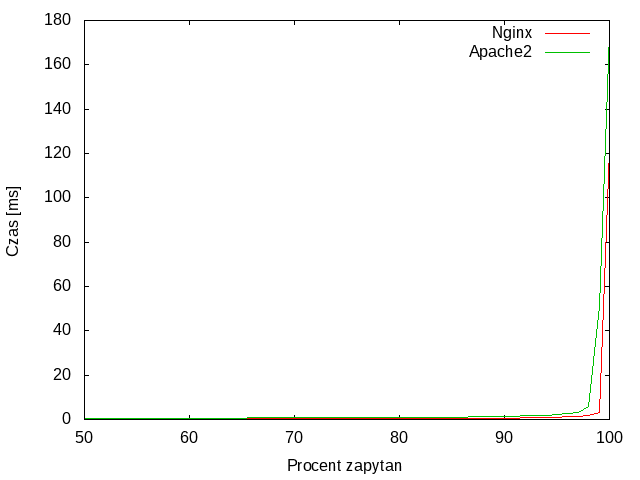
\includegraphics[width=\textwidth]{testy/wybor_index_maly_1.png}
		\caption{1 równoległe zapytanie}
	\end{subfigure}
	\begin{subfigure}[h]{0.3\textwidth}
		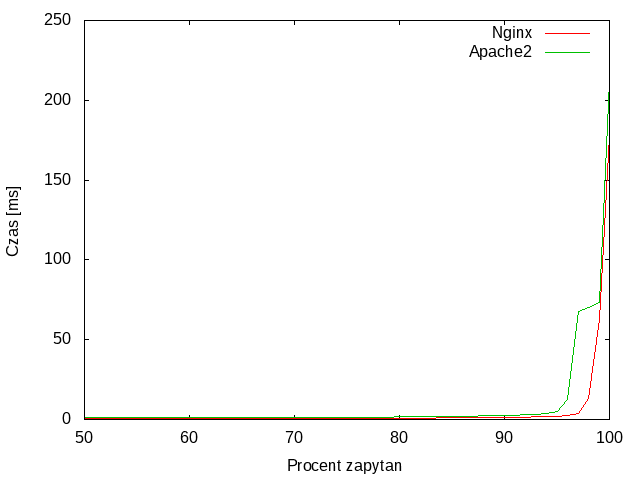
\includegraphics[width=\textwidth]{testy/wybor_index_maly_2.png}
		\caption{2 równoległe zapytania}
	\end{subfigure}
	\begin{subfigure}[h]{0.3\textwidth}
		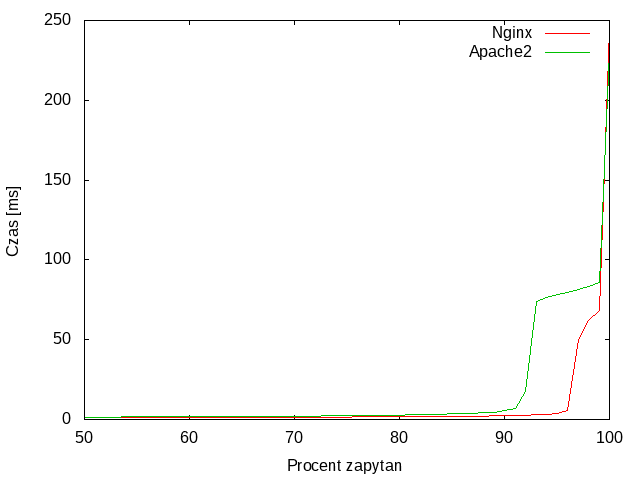
\includegraphics[width=\textwidth]{testy/wybor_index_maly_4.png}
		\caption{4 równoległe zapytania}
	\end{subfigure}

	\begin{subfigure}[h]{0.3\textwidth}
		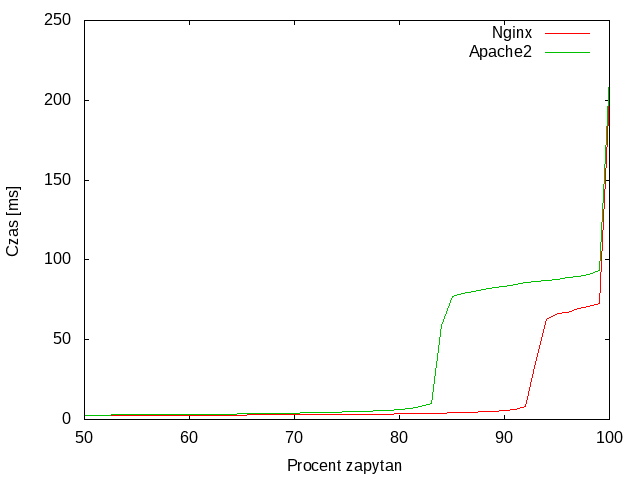
\includegraphics[width=\textwidth]{testy/wybor_index_maly_8.png}
		\caption{8 równoległych zapytań}
	\end{subfigure}
	\begin{subfigure}[h]{0.3\textwidth}
		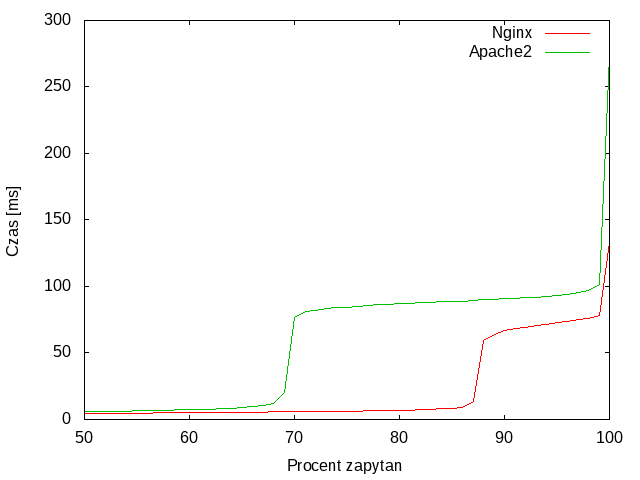
\includegraphics[width=\textwidth]{testy/wybor_index_maly_16.png}
		\caption{16 równoległych zapytań}
	\end{subfigure}
	\begin{subfigure}[h]{0.3\textwidth}
		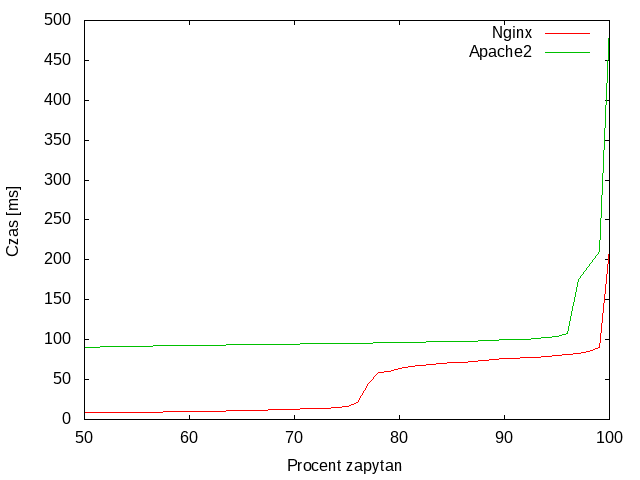
\includegraphics[width=\textwidth]{testy/wybor_index_maly_32.png}
		\caption{32 równoległe zapytania}
	\end{subfigure}

	\begin{subfigure}[h]{0.3\textwidth}
		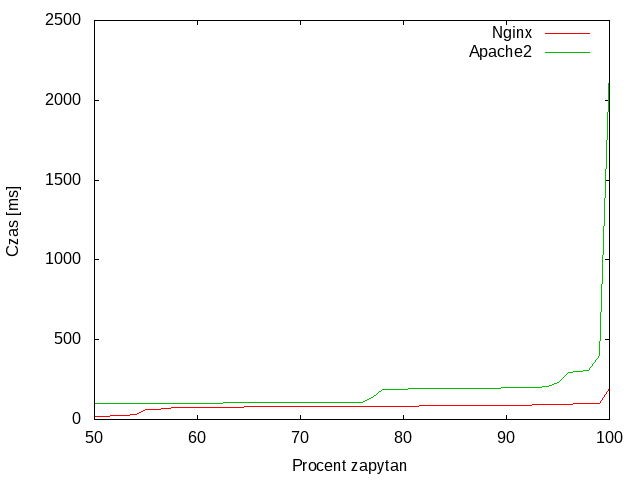
\includegraphics[width=\textwidth]{testy/wybor_index_maly_64.png}
		\caption{64 równoległe zapytania}
	\end{subfigure}
	\begin{subfigure}[h]{0.3\textwidth}
		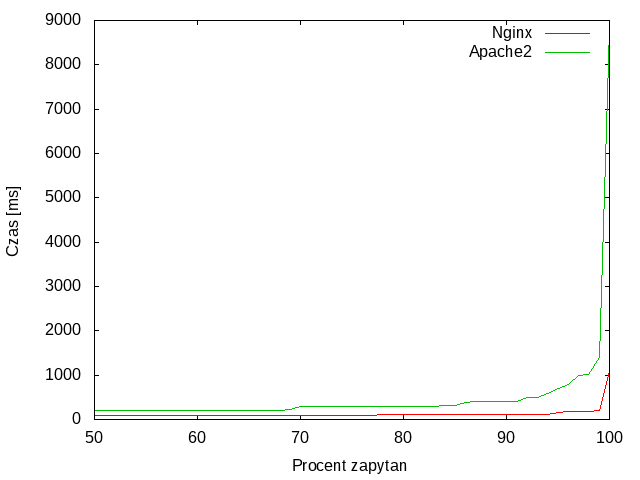
\includegraphics[width=\textwidth]{testy/wybor_index_maly_128.png}
		\caption{128 równoległe zapytania}
	\end{subfigure}
	\begin{subfigure}[h]{0.3\textwidth}
		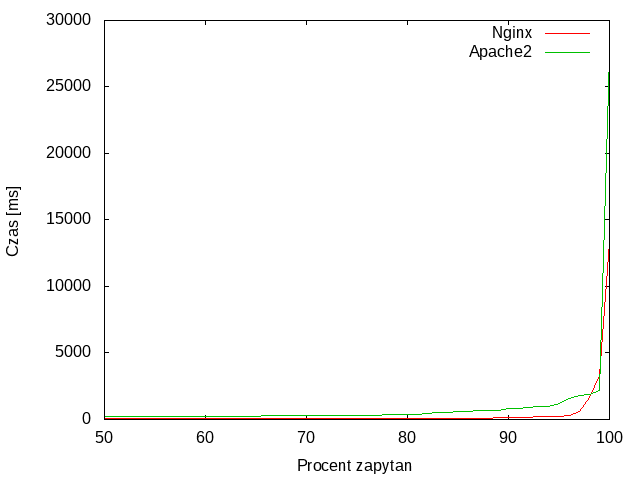
\includegraphics[width=\textwidth]{testy/wybor_index_maly_256.png}
		\caption{256 równoległych zapytań}
	\end{subfigure}
	\caption{Zapytania o mały plik statyczny}\label{fig:wyb_index_maly}
\end{figure}
\begin{figure}
	\centering
	\begin{subfigure}[h]{0.3\textwidth}
		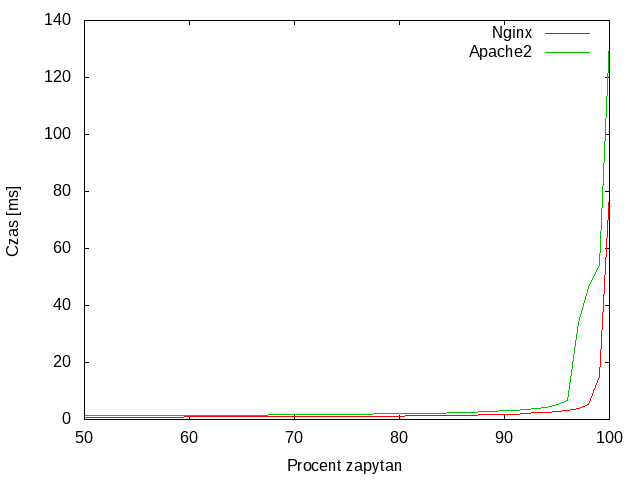
\includegraphics[width=\textwidth]{testy/wybor_index_duzy_1.png}
		\caption{1 równoległe zapytanie}
	\end{subfigure}
	\begin{subfigure}[h]{0.3\textwidth}
		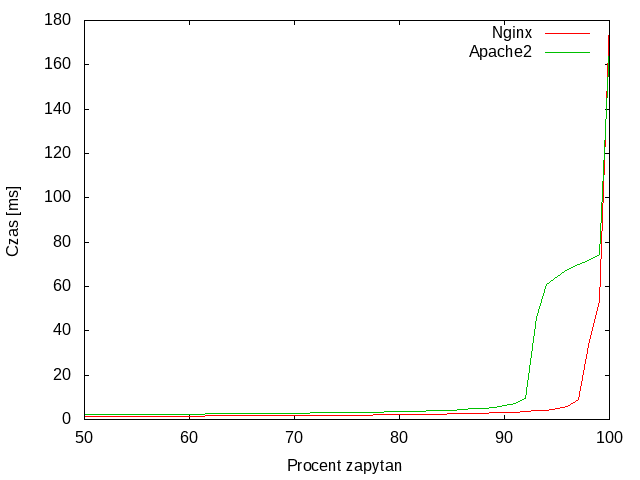
\includegraphics[width=\textwidth]{testy/wybor_index_duzy_2.png}
		\caption{2 równoległe zapytania}
	\end{subfigure}
	\begin{subfigure}[h]{0.3\textwidth}
		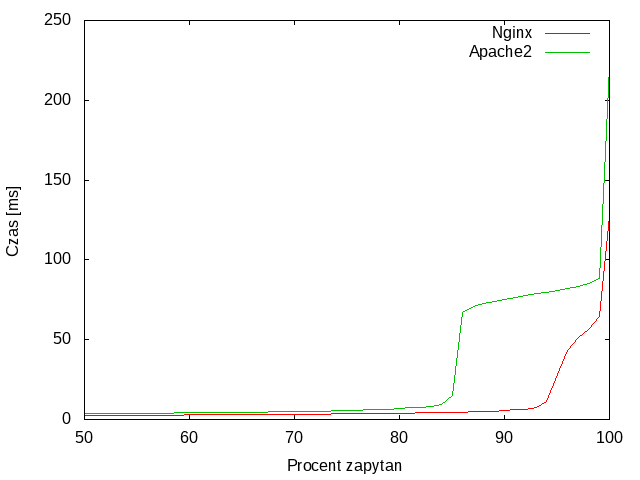
\includegraphics[width=\textwidth]{testy/wybor_index_duzy_4.png}
		\caption{4 równoległe zapytania}
	\end{subfigure}

	\begin{subfigure}[h]{0.3\textwidth}
		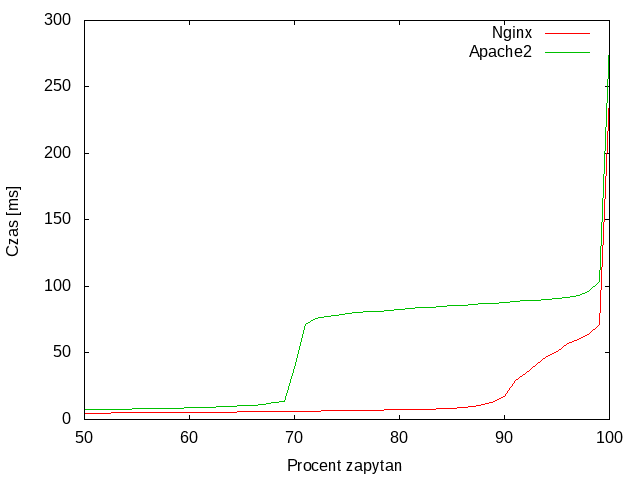
\includegraphics[width=\textwidth]{testy/wybor_index_duzy_8.png}
		\caption{8 równoległych zapytań}
	\end{subfigure}
	\begin{subfigure}[h]{0.3\textwidth}
		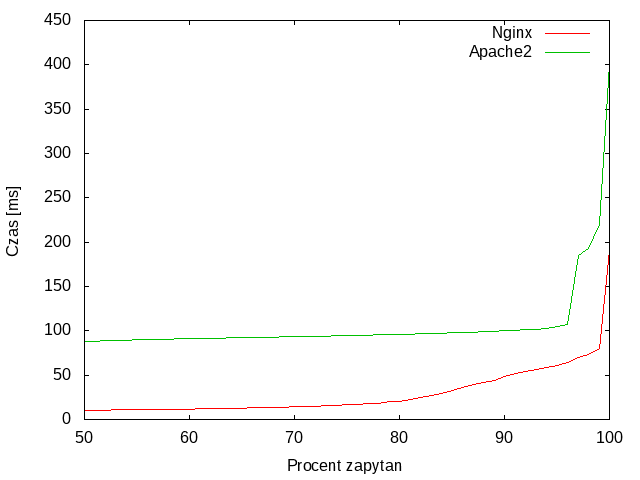
\includegraphics[width=\textwidth]{testy/wybor_index_duzy_16.png}
		\caption{16 równoległych zapytań}
	\end{subfigure}
	\begin{subfigure}[h]{0.3\textwidth}
		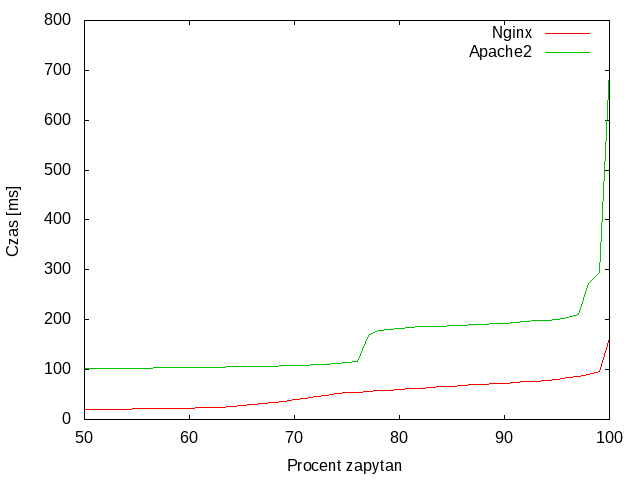
\includegraphics[width=\textwidth]{testy/wybor_index_duzy_32.png}
		\caption{32 równoległe zapytania}
	\end{subfigure}

	\begin{subfigure}[h]{0.3\textwidth}
		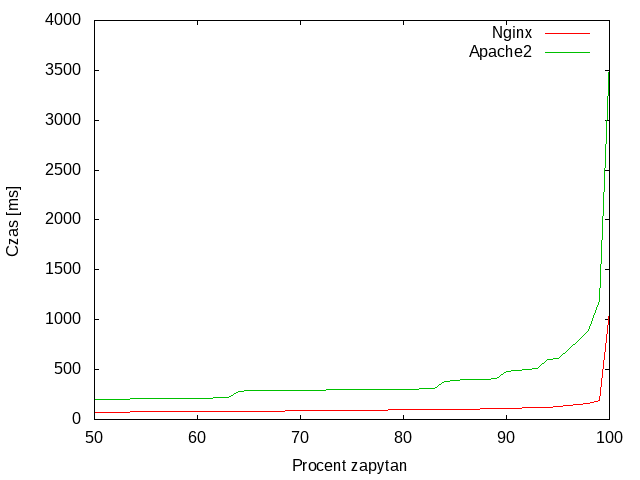
\includegraphics[width=\textwidth]{testy/wybor_index_duzy_64.png}
		\caption{64 równoległe zapytania}
	\end{subfigure}
	\begin{subfigure}[h]{0.3\textwidth}
		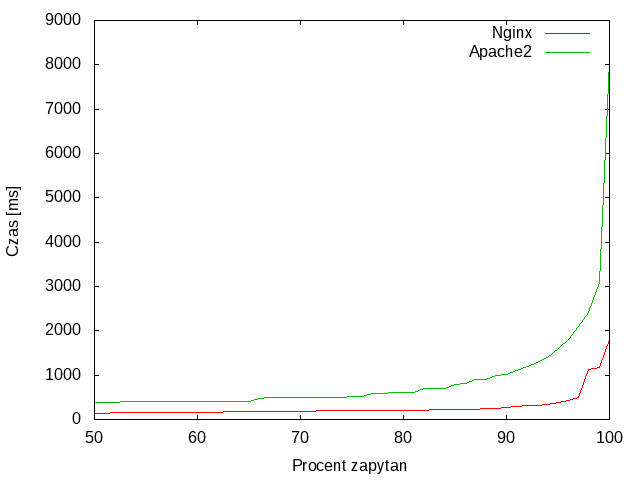
\includegraphics[width=\textwidth]{testy/wybor_index_duzy_128.png}
		\caption{128 równoległe zapytania}
	\end{subfigure}
	\begin{subfigure}[h]{0.3\textwidth}
		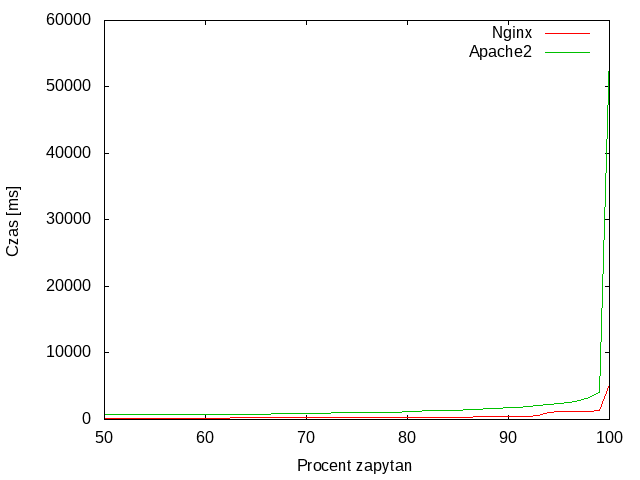
\includegraphics[width=\textwidth]{testy/wybor_index_duzy_256.png}
		\caption{256 równoległych zapytań}
	\end{subfigure}
	\caption{Zapytania o duży plik statyczny}\label{fig:wyb_index_duzy}
\end{figure}
Wykresy na rys.~\ref{fig:wyb_index_maly} przedstawiają czasy obsłużenia zapytań o plik HTML o rozmiarze 10 bajtów, natomiast wykresy na rys.~\ref{fig:wyb_index_duzy} czasy zapytań o plik o rozmiarze 100 kilobajtów.

Można zauważyć, że wyniki dla małych plików statycznych są zbliżone zarówno dla Apache jak i Nginx z lekką przewagą dla Nginx.
Największą przewagę Nginxa widać przy średnim i dużym obciążeniu.
\clearpage
\subsection{Treść dynamiczna}
Testy treści dynamicznej przeprowadzane są przy użyciu konfiguracji Nginx + php-fpm oraz Apache + php-fpm.
Konfiguracja Apache + mod\_php została odrzucona, ponieważ wymaga umieszczenia serwera WWW oraz serwera PHP na jednym serwerze, co uniemożliwia użycie wielu serwerów PHP dla jednego serwera WWW.

Do testów zostały wykorzystane dwa bliźniacze skrypty obliczające liczby ciągu Fibonacciego.
Jeden ze skryptów został przedstawiony na listingu~\ref{lst:fib}.
Obliczane są wyrazy: piąty --- dla skryptu wykonującego się szybko, oraz piętnasty --- dla skryptu wykonującego się dłużej.

Wykorzystany został rwkurencyjny model obliczanie wartości, ponieważ w przeciwieństwie do iteracyjnego wymaga większej mocy obliczeniowej.
Pożądane jest, aby czas obsługi zapytania obejmował czas wykonywania skryptu, a nie jedynie obsługi sesji HTTP oraz transferu danych (zostało to przetestowane przy wykorzystaniu \textit{szybkiego skryptu}).
\lstinputlisting[caption=fib.php,label=lst:fib,language=php]{lst/fib.php}
\begin{figure}
	\centering
	\begin{subfigure}[h]{0.3\textwidth}
		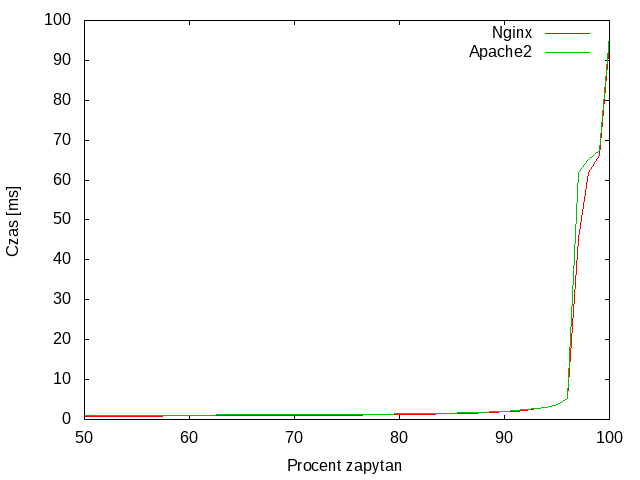
\includegraphics[width=\textwidth]{testy/wybor_fib_5_1.png}
		\caption{1 równoległe zapytanie}
	\end{subfigure}
	\begin{subfigure}[h]{0.3\textwidth}
		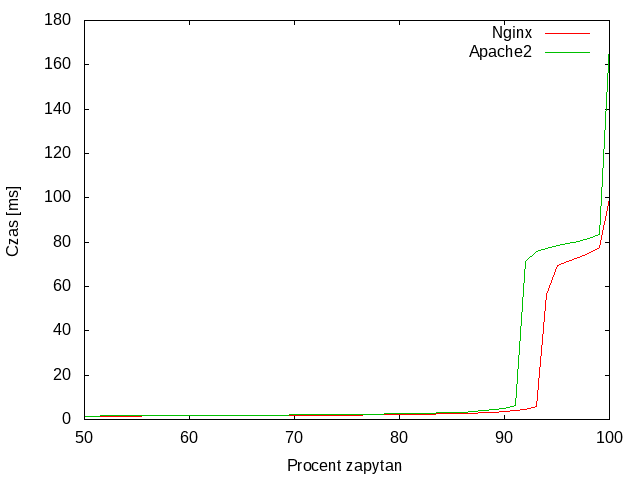
\includegraphics[width=\textwidth]{testy/wybor_fib_5_2.png}
		\caption{2 równoległe zapytania}
	\end{subfigure}
	\begin{subfigure}[h]{0.3\textwidth}
		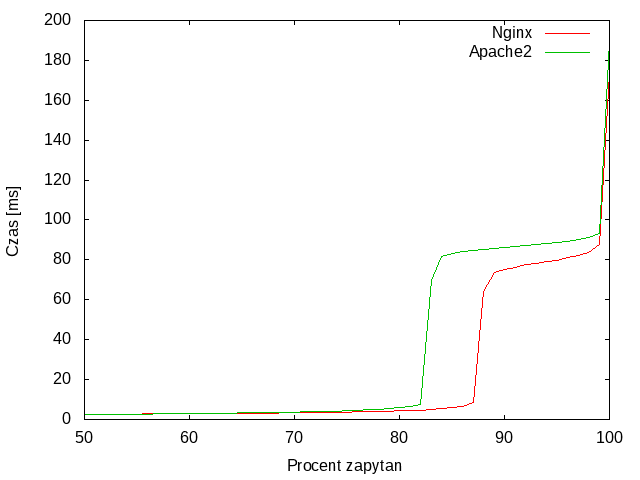
\includegraphics[width=\textwidth]{testy/wybor_fib_5_4.png}
		\caption{4 równoległe zapytania}
	\end{subfigure}

	\begin{subfigure}[h]{0.3\textwidth}
		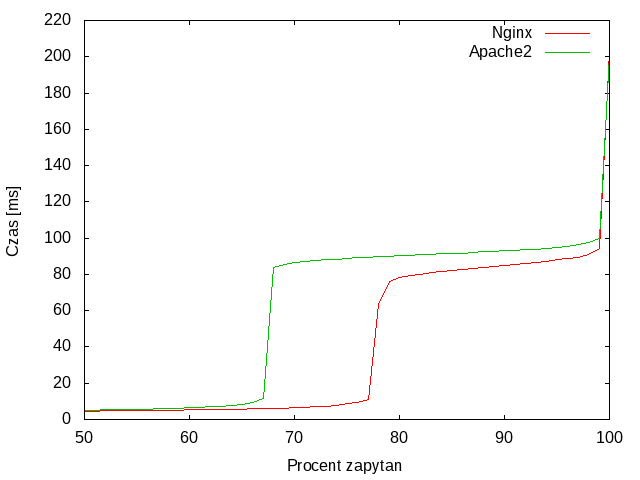
\includegraphics[width=\textwidth]{testy/wybor_fib_5_8.png}
		\caption{8 równoległych zapytań}
	\end{subfigure}
	\begin{subfigure}[h]{0.3\textwidth}
		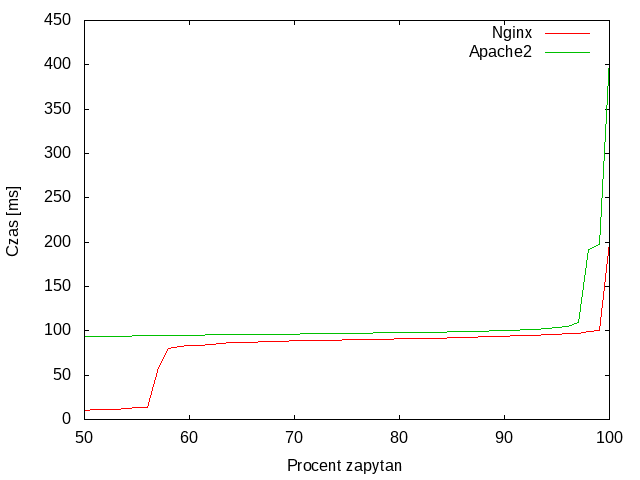
\includegraphics[width=\textwidth]{testy/wybor_fib_5_16.png}
		\caption{16 równoległych zapytań}
	\end{subfigure}
	\begin{subfigure}[h]{0.3\textwidth}
		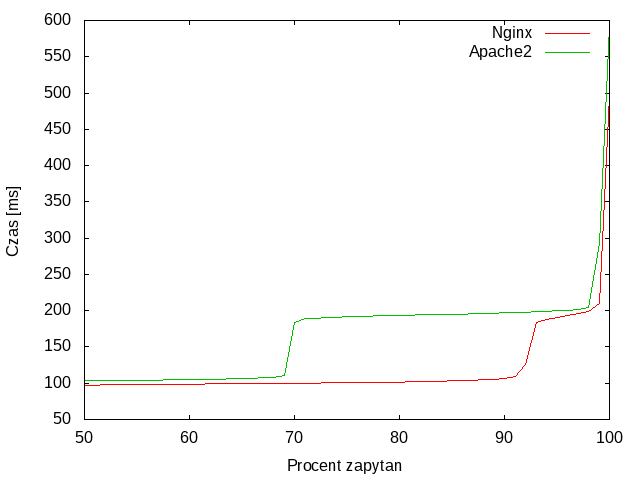
\includegraphics[width=\textwidth]{testy/wybor_fib_5_32.png}
		\caption{32 równoległe zapytania}
	\end{subfigure}

	\begin{subfigure}[h]{0.3\textwidth}
		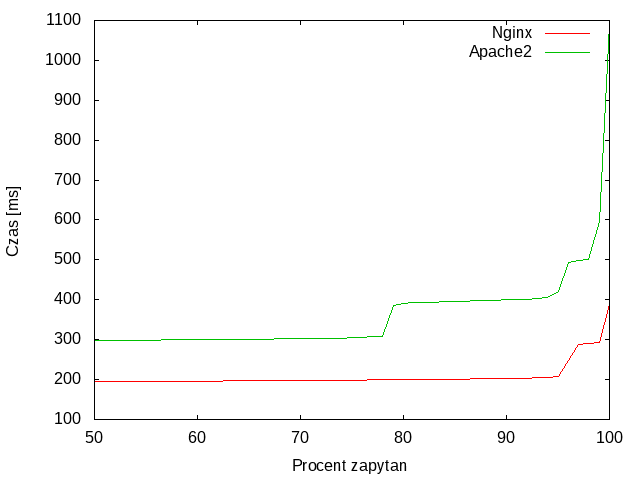
\includegraphics[width=\textwidth]{testy/wybor_fib_5_64.png}
		\caption{64 równoległe zapytania}
	\end{subfigure}
	\begin{subfigure}[h]{0.3\textwidth}
		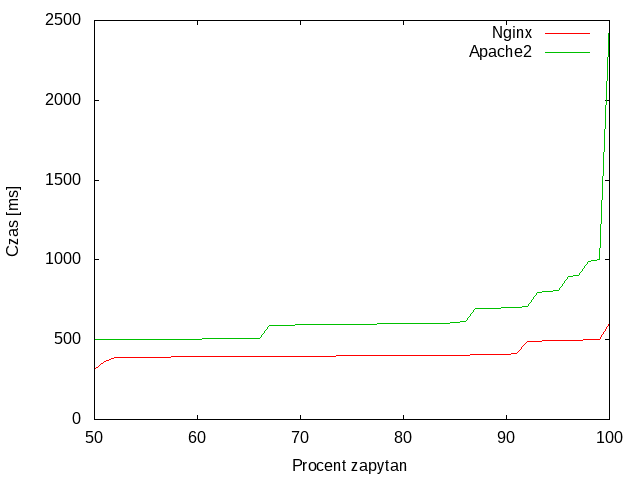
\includegraphics[width=\textwidth]{testy/wybor_fib_5_128.png}
		\caption{128 równoległe zapytania}
	\end{subfigure}
	\begin{subfigure}[h]{0.3\textwidth}
		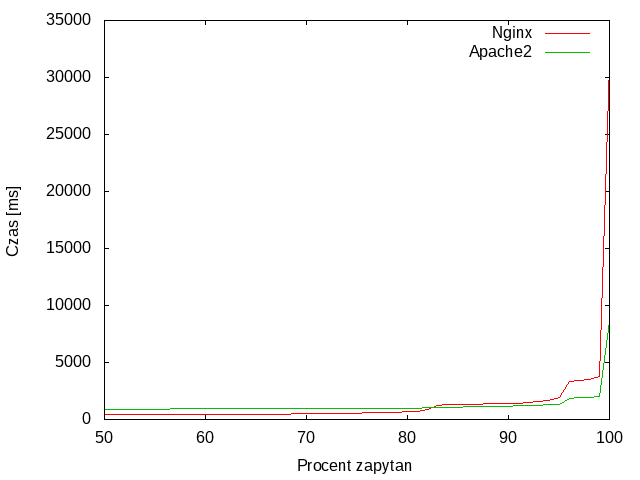
\includegraphics[width=\textwidth]{testy/wybor_fib_5_256.png}
		\caption{256 równoległych zapytań}
	\end{subfigure}
	\caption{Zapytania o szybki skrypt PHP}\label{fig:wyb_fib_5}
\end{figure}
\begin{figure}
	\centering
	\begin{subfigure}[h]{0.3\textwidth}
		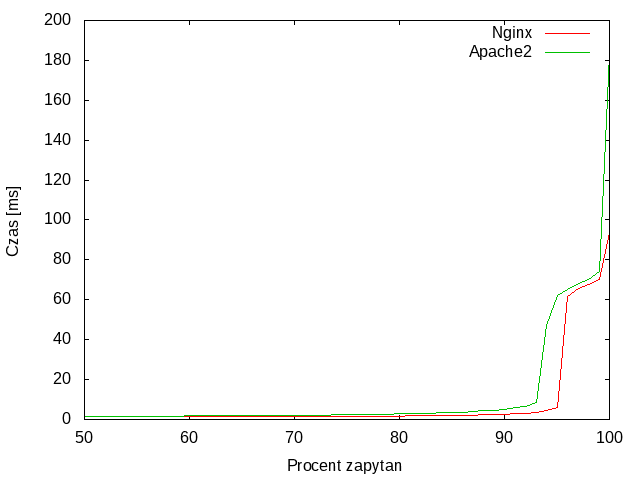
\includegraphics[width=\textwidth]{testy/wybor_fib_15_1.png}
		\caption{1 równoległe zapytanie}
	\end{subfigure}
	\begin{subfigure}[h]{0.3\textwidth}
		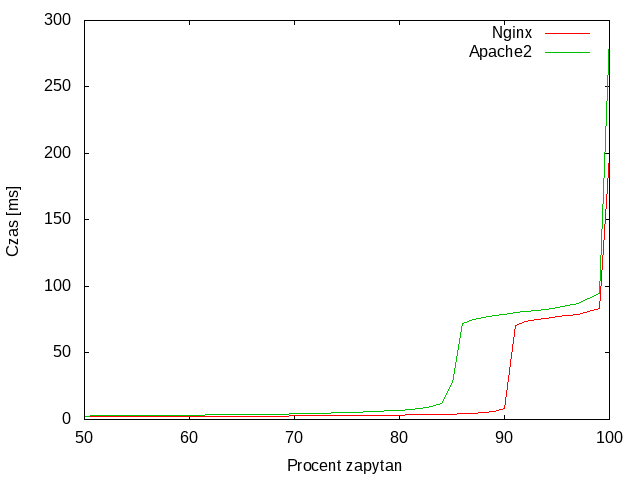
\includegraphics[width=\textwidth]{testy/wybor_fib_15_2.png}
		\caption{2 równoległe zapytania}
	\end{subfigure}
	\begin{subfigure}[h]{0.3\textwidth}
		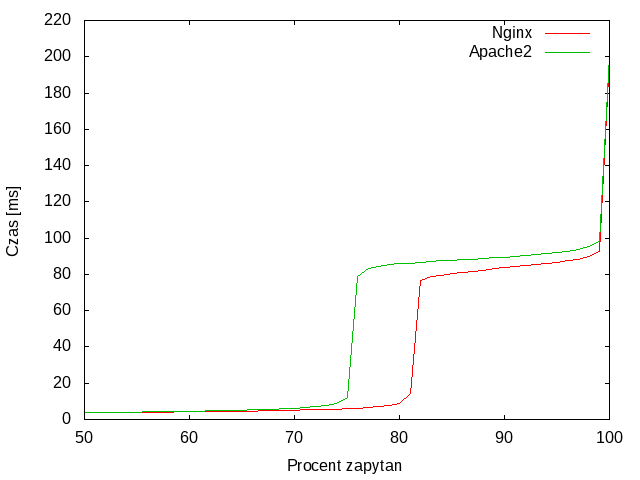
\includegraphics[width=\textwidth]{testy/wybor_fib_15_4.png}
		\caption{4 równoległe zapytania}
	\end{subfigure}

	\begin{subfigure}[h]{0.3\textwidth}
		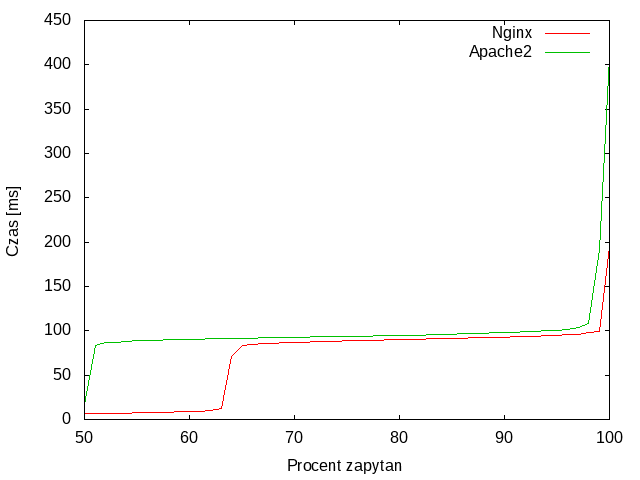
\includegraphics[width=\textwidth]{testy/wybor_fib_15_8.png}
		\caption{8 równoległych zapytań}
	\end{subfigure}
	\begin{subfigure}[h]{0.3\textwidth}
		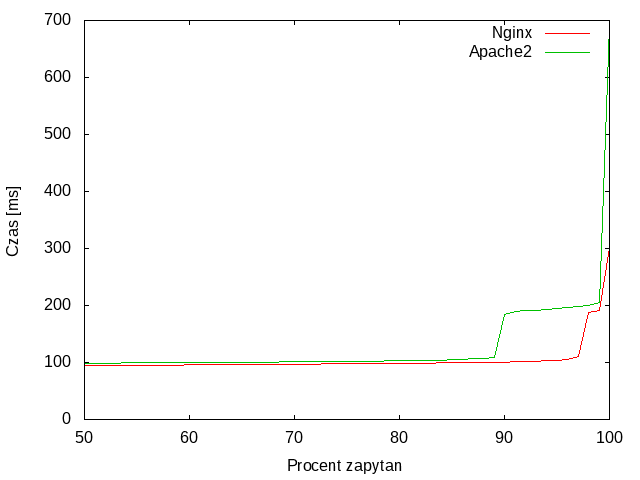
\includegraphics[width=\textwidth]{testy/wybor_fib_15_16.png}
		\caption{16 równoległych zapytań}
	\end{subfigure}
	\begin{subfigure}[h]{0.3\textwidth}
		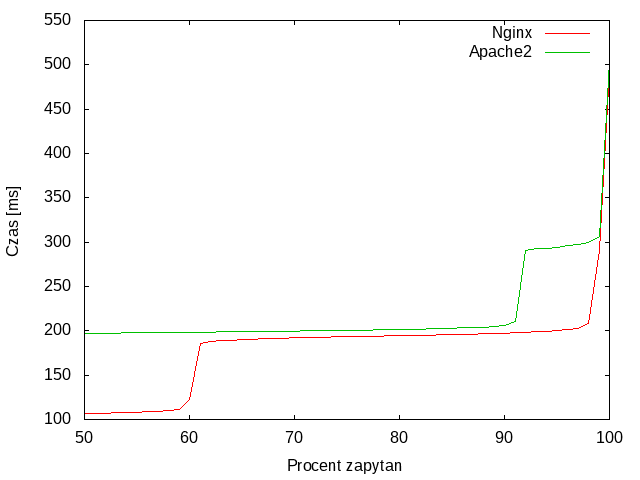
\includegraphics[width=\textwidth]{testy/wybor_fib_15_32.png}
		\caption{32 równoległe zapytania}
	\end{subfigure}

	\begin{subfigure}[h]{0.3\textwidth}
		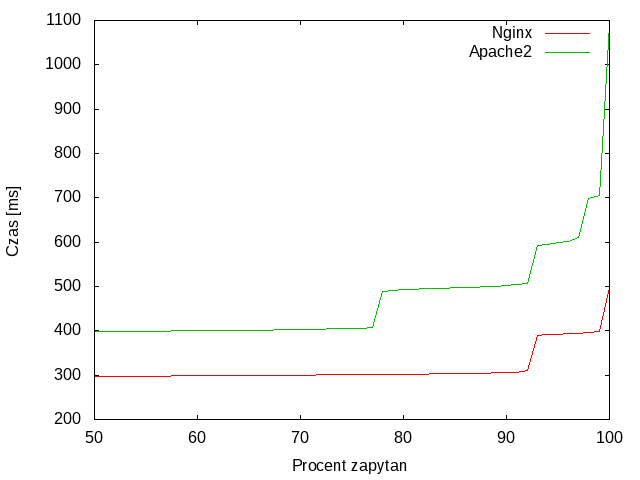
\includegraphics[width=\textwidth]{testy/wybor_fib_15_64.png}
		\caption{64 równoległe zapytania}
	\end{subfigure}
	\begin{subfigure}[h]{0.3\textwidth}
		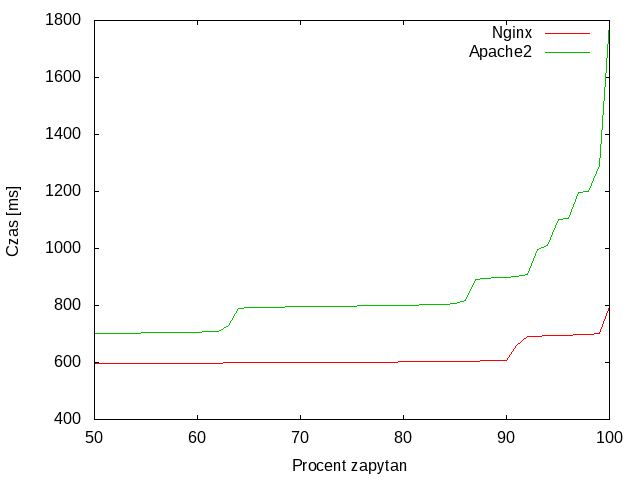
\includegraphics[width=\textwidth]{testy/wybor_fib_15_128.png}
		\caption{128 równoległe zapytania}
	\end{subfigure}
	\begin{subfigure}[h]{0.3\textwidth}
		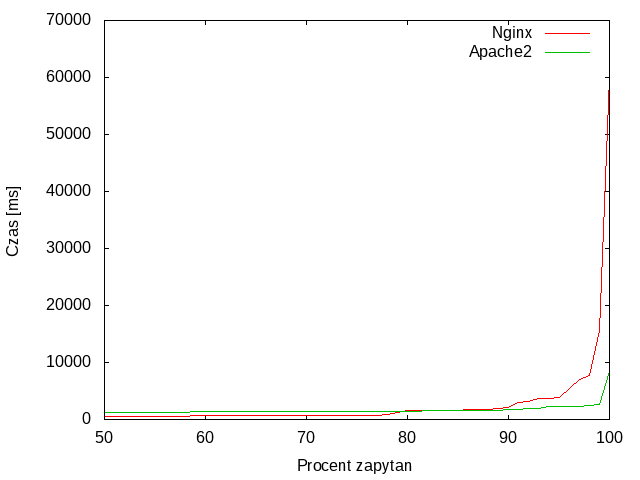
\includegraphics[width=\textwidth]{testy/wybor_fib_15_256.png}
		\caption{256 równoległych zapytań}
	\end{subfigure}
	\caption{Zapytania o wolny skrypt PHP}\label{fig:wyb_fib_15}
\end{figure}
Na wykresach~\ref{fig:wyb_fib_5} oraz~\ref{fig:wyb_fib_15} obrazujących czasy obsługi zapytań do skryptów PHP można zauważyć że różnice pomiędzy Apache a Nginx są mniejsze niż dla plików statycznych.
Wynika to z faktu, że obsługą zapytań w obu przypadkach zajmuje się PHP-fpm, natomiast serwer WWW odpowiedzialny jest jedynie za przekazywanie zapytań do \textit{backendu}.
\subsection{Podsumowanie}
Jak wykazały testy, Nginx daje krótsze czasy odpowiedzi we wszystkich testowanych sytuacjach, dlatego został wybrany jako podstawowy serwer wykorzystywany w przedstawionym projekcie.
\clearpage
\section{DNS round robin}
\subsection{Uwagi wstępne}
Jak zostało wspomniane w rozdziale~\ref{sec:dns} DNS round robin nie jest metodą \textit{load balancingu} a jedynie wstępną metodą dystrybucji ruchu.
Pociąga to za sobą pewne konsekwencje.
Przeciętna aplikacja sieciowa, np: Chrome bądź Links, dokonuje rozwiązania nazwy przy pierwszym odwołaniu się do danego adresu a następnie w celu zwiększenia wydajności \textit{cachuje} jej adres.
Efektem takiego zachowania jest nawiązywanie późniejszych połączeń do tego samego adresu IP\@.
Aplikacja \textit{Apache Benchmark}, która jest wykorzystywana do testowania rozwiązań w niniejszej pracy, również dokonywała jednorazowego rozwiązania nazwy i łączenia się do jednego adresu, co uniemożliwiało przeprowadzenie testów wydajnościowych \textit{DNS round robin} przy użyciu tego narzędzia.
Została zgłoszona korekta \cite{ab_dnsrr} poprawiająca tę niedogodność.
Testy z wykorzystaniem tej poprawki symulują łączenie się dużej liczby niezależnych użytkowników.

Przy testowanie \textit{DNS round robin} nie zostanie przeprowadzona tak dokładna analiza jak przy wyborze serwera WWW, ponieważ metoda ta nie wpływa na działanie serwera WWW a jedynie na dystrybucję ruchu.

W testach tych, w przeciwieństwie do wyboru serwera WWW, użyto opcji \texttt{Keep Alive} powodującej utrzymywanie i wykonywanie kolejnych połączeń bez ponownego nawiązywania połączeń TCP\@.
W przypadku użycia poprawki~\cite{ab_dnsrr} każde połączenie jest tworzone do serwera wynikającego z technologi \textit{DNS round robin} a następnie jest ono utrzymywane aż do zakończenia programu. Liczba połączeń zależy od parametru \texttt{concurrent}.
\subsection{Testy wydajnościowe}
Testowanie rozwiązania \textit{DNS round robin} zostanie przedstawione na odpytywaniu jedynie pliku statycznego, ponieważ testy dla pozostałych treści będą analogiczne do tych przedstawionych w rozdziale~\ref{sec:wybor}.

Do testów został wykorzystany \textit{DNS round robin} przedstawiony na listingu~\ref{lst:test_dnsrr}.
\lstinputlisting[caption=DNS round robin, label=lst:test_dnsrr]{lst/test_dnsrr.bash}
Zawiera on cztery serwery z identyczną konfiguracją.\\
Wykresy~\ref{fig:test_dnsrr} przedstawiają czasy obsługi zapytań w przypadku pojedynczego serwera WWW oraz grupy serwerów z dystrybucją ruchu poprzez \textit{DNS round robin}.
Na wykresach został pominięty czas najdłuższego połączenia z powodu małego wkładu informacyjnego oraz dużego stopnia zaciemniania obrazu.
\wykresy{dnsrr}{Dystrybuja ruchu w oparciu o DNS RR}{test_dnsrr}
Tabela~\ref{tab:test_dnsrr} przedstawia liczbę obsłużonych zapytań na sekundę.
\begin{table}[h]
\centering
\begin{tabular}{cccc}
	\toprule
	Liczba połączeń & Nginx & DNS RR & Przyrost\\
	\midrule
	\midrule
	1&2571&4301& +67\%\\
	\midrule
	2&2001&5458& +172\%\\
	\midrule
	4&1353&6264& +362\%\\
	\midrule
	8&1704&7582& +344\%\\
	\midrule
	16&2097&8720& +315\%\\
	\midrule
	32&2133&7484& +250\%\\
	\midrule
	64&1968&10617& +439\%\\
	\midrule
	128&1945&10194& +424\%\\
	\midrule
	256&2190&9821& +348\%\\
	\bottomrule
\end{tabular}
\caption{Obsłużonych zapytań na sekundę}
\label{tab:test_dnsrr}
\end{table}
\subsection{Podsumowanie}
Jak można zaobserwować na wykresach, użycie dystrybucji ruchy zmniejsza czasy oczekiwania na przetworzenie zapytań.

Dane przedstawione w tabeli~\ref{tab:test_dnsrr} pokazują, iż użycie czterech serwerów zamiast jednego daje w większości przypadków przyrost ok. 300\%, co jest wartością oczekiwaną, ponieważ przy użyciu trzech dodatkowych serwerów spodziewamy się trzykrotnego przyrostu wydajności.

W przypadku jednego równoległego połączenia oczekiwanym przyrostem były przyrost 0\%, ponieważ wykonywane jest jedno połączenie, jednak specyfika serwera Nginx jest taka, że po przyjęciu stu połączeń w trybie \texttt{Keep-Alive} zamyka on połączenie.
Następuje wtedy nawiązanie kolejnego, które zostaje przekierowane do kolejnego serwera z puli \textit{DNS round robin}.
Jest to przyczyną zwiększonego przyrostu dla jednego i dwóch równoległych połączeń.

Przy liczbie czterech i więcej połączeń powyższy efekt nie ma znaczenia, ponieważ w obsłudze zapytań biorą udział wszystkie serwery.
\section{LVS}
W tej sekcji przetestowany zostanie LVS w trybie \textit{direct routing}.
Testom poddany zostanie narzut wynikający z użycia LVS, jak również przetestowane zostaną rozwiązanie bliższe rzeczywistości, czyli zawierające kilka \textit{real serverów}.
Ponadto sprawdzone zostanie zachowanie LVS w warunkach nieidealnych, tj.\ w przypadku awarii jednego z \textit{real serverów} oraz w przypadku wysycenia łącza.
\subsection{Uwagi dotyczące urządzeń sieciowych}
\label{sub:uwagi_sieciowe}
Ponieważ w omawianym rozwiązaniu występuje jeden węzeł, do którego nawiązywane są połączenia, parametry łącza są w tym przypadku istotne (w przeciwieństwie do DNS round robin gdzie klient łączy się do różnych serwerów).
\begin{description}
	\item{Maszyna z \textit{directorem}:}
		\begin{itemize}
			\item Wirtualizowany sterownik karty sieciowej: rtl8139
			\item Szybkość karty podawana przez ethtool: 100Mb/s
		\end{itemize}
	\item{Maszyna z LXC:}
		\begin{itemize}
			\item Wirtualizowany sterownik karty sieciowej: virtio
			\item Szybkość karty podawana przez ethtool: Brak
		\end{itemize}
	\item{Maszyna z Nginx}
		\begin{itemize}
			\item Wirtualizowany sterownik karty sieciowej: wirtualny interface hosta
			\item Szybkość karty podawana przez ethtool: 10000Mb/s
		\end{itemize}
\end{description}
Na uwagę zasługują tutaj parametry maszyny będącej hostem dla LXC\@.
Użycie sterownika \texttt{virtio} pozwala maszynie wirtualizowanej komunikować się z maszyną hostującą bez emulacji konkretnych sterowników sieciowych, lecz już na poziomie jądra.
Dlatego nie jest możliwe określenie prędkości takiego interface'u, ponieważ zasada jego działania jest inna niż rzeczywistych kart sieciowych.

Podobnie sytuacja wygląda dla kontenerów LXC\@.
Tam komunikacja następuje poprzez wirtualne interface'y na jednej maszynie, dlatego prędkość podana przez \texttt{ethtool} wynosi 10Gb/s.

W przypadku testowania zachowania rozwiązania na wysycenie łącza, prędkość interface'u na maszynie z \textit{directorem} zostanie ustawiona na 10Mb/s.
Pozwoli to zasymulować sytuację, w której żądany ruch będzie większy niż możliwości łącza serwera.
\subsection{Narzut własny LVS}
\label{sec:lvs_narzut}
Aby sprawdzić jakie opóźnienie generuje mechanizm LVS, skonfigurowany zostanie jeden serwer \textit{director} oraz jeden \textit{real server}.
Porównując czasy odpowiedzi serwera WWW odpytywanego bezpośrednio oraz poprzez LVS, otrzymamy jaki wpływ na działanie ma LVS\@.
Żądany będzie mały plik statyczny.
\wykresy{one_lvs_maly}{Narzut własny LVS}{one_lvs_maly}

Jak widać na rysunku~\ref{fig:one_lvs_maly} czasy odpowiedzi serwera bezpośrednio oraz poprzez LVS nie odbiegają zbytnio od siebie.
Różnica na wykresie jest widoczna jedynie dla jednego konkurencyjnego zapytania, jednak wartości tych czasów (0.2ms i 0.4ms) są na tyle małe, że ta różnica może zostać pominięta.
\subsection{Wiele real serverów}
Rozważmy teraz przypadek, w którym mamy cztery takie same serwery WWW\@.
Zostały skonfigurowane 3 usługi LVS\@. Tę konfigurację przedstawia listing~\ref{lst:four_lvs_maly}.
\footnotesize
\lstinputlisting[caption=LVS z wieloma serwerami,label=lst:four_lvs_maly]{lst/four_lvs_maly}
\normalsize
Widzimy, że każda z usług posiada inną liczę serwerów oraz taki sam algorytm balansowania.
Każdy z serwerów ma wagę 1 oraz każdy jest wykorzystywany w trybie \textit{direct routing}.

\wykresy{four_lvs_maly}{Czasy odpowiedzi w zależności od ilości serverów}{four_lvs_maly}
Wykresy~\ref{fig:four_lvs_maly} przedstawiają czasy odpowiedzi w zależności o ilości \textit{real serverów}.
Wymaga to trochę dokładniejszej analizy niż poprzednie wykresy.
Dla jednego równoległego zapytania widzimy, że czasy każdej z usług LVS są gorsze niż bezpośrednie zapytania do server WWW\@.
Dzieje się tak dlatego, że mając jedno równoczesne zapytanie, wykorzystywany jest tylko jeden serwer na raz, czyli jest to sytuacja tożsama z tą występującą w rozdziale~\ref{sec:lvs_narzut}.
W przypadku 2 połączeń wykresy zaczynają się zbiegać, ponieważ narzut LVS jest kompensowany poprzez dystrybucję zapytań.

Począwszy od czterech zapytań zauważamy, że połączenia kierowane do LVS są obsługiwane szybciej.
Najbardziej jest to widoczne przy dużym obciążeniu serwera, tj. 128 i 256 równoległych zapytań.

\chapter{Opis projektu}
\section{Opis}
W poprzednich rozdziałach zostały przedstawione metody klastrowania oraz zarządzania konfiguracją, a następnie zostały one przetestowane.
Została również wykazana zasadność ich stosowania.\\
Jednak, aby wdrożyć takie rozwiązania, potrzebna jest wiedza oraz czas pracy administratora.

\textit{System zautomatyzowanego zarządzania konfiguracją farmy serwerów aplikacji WWW} (zwany dalej \textit{SZZ}) ma za zadanie uprościć konfigurację klastra WWW, pozwalając zaoszczędzić czas i pieniądze.
Opisywany system będzie mógł być obsługiwany przez osoby nie posiadające dogłębnej wiedzy z zakresu administracji systemami linux ani serwerami WWW.
Wymagana jest jedynie podstawowa wiedza techniczna, którą posiada przeciętny programista.

Konfiguracja odbywa się poprzez edycję plików, dlatego obsługująca system powinna być w stanie obsługiwać połączenia \texttt{ssh} oraz edytor tekstowy.
\section{Struktura}
\textit{SZZ} wykorzystuje różne metody klastrowania.
Struktura systemu została przedstawiona na rys~\ref{fig:struktura}
\begin{figure}
	\centering
	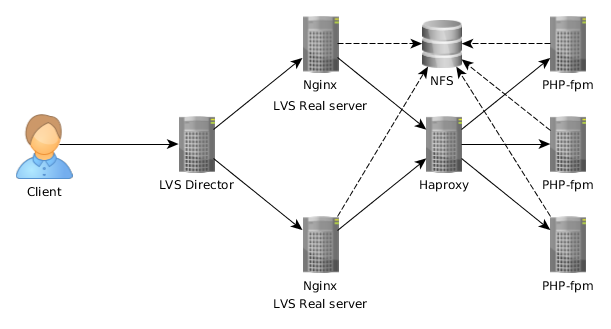
\includegraphics[width=\textwidth]{obrazy/struktura_szz.png}
	\caption{Struktura SZZ}
	\label{fig:struktura}
\end{figure}
Pierwszą warstwą klastrowania jest LVS (por.~\ref{sec:LVS}).
Zapytanie trafiające na serwer obsługiwane są przez \textit{direcotor}-a.
Następnie przekazywane są do serwerów WWW, które analizując zapytania serwują treści statyczne ze wspólnego zasobu NFS.
W przypadku zapytania o treści dynamiczne, zapytania przekazywane jest do warstwy trzeciej projektu, czyli usługi Haproxy, która przekazuje zadania do odpowiedniego serwera z usługą \textit{PHP-fpm}.
Po wygenerowaniu odpowiedzi, serwer roboczy zwraca odpowiedź do Haproxy, które przekazuje je do serwera WWW.
Ten natomiast, będąc \textit{real server}-em w klastrze LVS, odpowiada bezpośrednio klientowi.
\subsection{Warstwa zero - storage}
Projekt posiada wspólny zasób dyskowy wystawiany poprzez protokół NFS.
Metoda ta w znaczny sposób uprasza aktualizację aplikacji na wszystkich węzłach równocześnie - kosztem braku możliwości wykonywania tzw. \textit{rolling update}.
Ta technologi rozwiązuje również problem wgrywania plików na serwer oraz ich propagacji ponieważ każdy wgrywany plik trafia na wspólny zasób i jest od razu widziany przez pozostałe węzły.\\
Wydajność NFS jest zadowalająca przy wykorzystywaniu w obrębie jeden serwerowni i jednej sieci LAN.
W przypadku chęci użycia rozproszenia systemu między kilkoma \textit{datacenter} należy ze własnym zakresie obsłużyć synchronizację wgrywanych plików oraz aktualizacji.
\subsection{Warstwa pierwsza - LVS}
Jedynym wystawionym na świat serwerem jest \textit{director}. Do niego trafiają wszystkie zapytania od klientów.
Wykorzystana w projekcie konfiguracja używa \textit{scheduler}-a opartego o algorytm \textit{round robin}, czyli przekazuje zapytania na wszystkie serwery po kolei.
Technologia LVS pozwala na posiadanie tylko jednego serwera typu \textit{director}, ponieważ jego zadaniem jest jedynie przekazywanie zapytać do \textit{real server}-ów.
Ponadto, jak zostało omówione wcześniej, odpowiedzi do klienta wysyłane są bezpośrednio od \textit{real server}-ów, bez udziału \textit{director}-a co pozwala na obsługę nawet dużego ruchu.\\
Obecna konfiguracja nie posiada narzędzi do wykrywania niedostępności \textit{director}-a bądź \textit{real server}-ów, dlatego konfiguracja narzędzi typu \textit{heartbeat} oraz technologi \textit{floating IP} i/lub monitoringu stanu serwerów, leży po stronie użytkownika.
\subsection{Warstwa druga - Nginx}
Drugą warstwą jest warstwa serwerów WWW.
Do nich trafiają zapytania przekazywane z pierwszej warstwy.
Serwer WWW obsługujący wiele \textit{Virtual Host}-ów, analizuje zapytanie pod kontem, czy żądana ścieżka jest istniejącym plikiem na dysku.
Jeżeli plik istnieje, jest on serwowany klientowi.
W przeciwnym wypadku, zapytanie zostaje przekazywane do haproxy.
\subsection{Warstwa trzecia - Haproxy}
Haproxy jest trzecią warstwą systemu.
Przez tą warstwę przechodzą wszystkie zapytania o treści dynamiczne.
Usługa tworzy osobny \textit{frontend} oraz \textit{backend} dla każdego projektu.\\
Haproxy posiada wbudowaną obsługę wykrywania, dlatego warstwa trzecia zapewnia pełna \textit{HA}.\\
Wysycenie łącza dla warstwy trzeciej nie powinna być problemem, ponieważ zapytania odbywają się jedynie po dane dynamiczne - zwykle tekstowe.
Wszystkie zapytania o obrazy i inne treści statyczne zostają obsłużone warstwę wcześniej.
System nie zapewnia wysokiej dostępności dla usługi haproxy.
Administrator powinien skonfigurować monitoring aby móc taką awarię wykryć maksymalnie szybko i usunąć usterkę.
W przypadku niemożliwości naprawy maszyny, system pozwala na skonfigurowanie nowej maszyny dla warstwy trzeciej oraz przekonfigurowanie w stosunkowo krótkim czasie.
\subsection{Warstwa czwarta - PHP-fpm}
Najniższą warstwą systemu jest warstwa robocza.
PHP-fpm odpowiedzialny jest za generowanie treści dynamicznych.
Podobnie jak serwer WWW, korzysta on ze współdzielonego zasobu dyskowego udostępnianego po NFS.
Na jednej maszynie może być uruchomionych kilka aplikacji PHP-fpm.
\section{Nazwa robocza: backend}
Sekcja ta opisuje kroki jakie podejmuje system, aby skonfigurować klaster zgodnie z założeniami.
\subsection{NFS}
Aby skonfigurować serwer NFS, system instaluje potrzebne pakiety a następnie kopiuje plik konfiguracyjny na serwer.
W następnej kolejności ustawia autostart server NFS oraz go uruchamia.\\
W drugiej kolejności, następuje instalacja \textit{git}-a.
Ostatnią wykonywaną rzeczą, jest \textit{deploy} wszystkich aplikacji.
\textit{Deploy} wykonywany jest do aktualnej wersji w gałęzi \textit{master}.
\subsection{Director}
Do skonfigurowania \textit{Directora}, potrzebna jest instalacja pakietu \texttt{ipvsadm}, który dostarcza narzędzia do konfiguracji \textit{Linux Virtual Server}.
Konfiguracja \textit{LVS} przeprowadzana jest poprzez użycie mechanizmu zapisu i odczytu aktualnej tablicy \textit{LVS}.
Tuż po instalacji, wykonywany jest zapis konfiguracji, w celu przeprowadzenia całej procedury zapisu tablicy do pliku.
Następnie, generowany jest nowy plik konfiguracji na podstawie parametrów zadanych przez użytkownika.
Plik ten jest wgrywany na serwer i podmienia poprzednio utworzony przy poleceniu zapisu.
Następnie wykonywana jest procedura wczytywania tablicy z pliku do aktualnie działającej instancji.
W efekcie, tablica wygenerowana przez system staje się aktualnie działającą.
Następnie ustawia się autouruchamianie usługi \texttt{LVS}.\\
W drugiej kolejności, tworzony jest wirtualny interface sieciowy, oraz zostają mu przypisane adresy IP odpowiednie dla konkretnych projektów.\\
Każdy projekt nasłuchuje na dedykowanym sobie adresie IP.
Daje to możliwość dedykowania konkretnych serwerów WWW dla projektów, zamiast przypisywać obsługę wszystkich serwerów dla każdego projektu.
\subsection{Real server}
Konfiguracja \textit{real server}-ów jest zbliżona do \textit{director}-a.
Następuje stworzenie wirtualnego interface-u a następnie przypisanie mu odpowiednich adresów IP.
Ważną różnicą w przypadku \textit{real server}-ów jest zapewnienie, aby \textit{real server}-y nie odpowiadały na zapytania \texttt{ARP}.
Uzyskiwane jest to poprzez użycie \texttt{arptables}.
System blokuje wszystkie pakiety typu \textit{ARP response} i pochodzące z adresacji używanej przez \textit{LVS} do nasłuchiwania przez projekty.
\subsection{Server WWW}
Serwer WWW instalowany jest na \textit{real server}-rze.
Następuje instalacja serwera \texttt{nginx} oraz ustawienie jego autouruchamiania.\\
W kolejnym kroku generowana jest konfiguracja \textit{vhost}-ów.
Dla każdej \textit{hostgroup}-y z konfiguracji, zaczynającej się od \textit{proj\_} (założenie konfiguracji), tworzona jest osobna sekcja \texttt{server}.
\texttt{Document root} jest ustawiany do odpowiedniego katalogu na zasobie sieciowym.
Następnie konfigurowane jest \textit{proxy} plików \texttt{php} do serwera z odpowiednio skonfigurowanym \textit{haproxy}.\\
Obecna wersja oprogramowania nie wspiera przyjaznych linków, prowadzących do skryptów PHP a nie kończących się rozsrzerzeniem \texttt{.php}.
\subsection{Server haproxy}
Konfiguracja serwera haproxy polega, podobnie jak innych komponentów, na instalacji aplikacji, wgraniu konfiguracji oraz uruchomieniu usługi.
System tworzy konfigurację dla haproxy bazując na ustawieniach projektów użytkownika.
Dla każdego zdefiniowanego w systemie projektu, \texttt{backend}, wykorzystujący algorytm \textit{round robin}, a następnie umieszcza w nim wszystkie serwery typu \texttt{worker} odpowiedzialne za procesowany projekt.
Następnie tworzy \texttt{frontend} nasłuchujący na porcie odpowiadającym \textit{id} projetu oraz wykorzystujący odpowiedni \texttt{backend}\\
Dodatkowo, \textit{haproxy} wystawia na standardowym porcie $9000$ statystyki aktualnie działającej instancji.

\addcontentsline{toc}{chapter}{Podsumowanie}
\chapter*{Podsumowanie}
Niniejsza praca wykazała potrzebę stosowania klastrów WWW.
Przy obecnym rozwoju internetu, ilość zapotrzebowania na dane jest daleko wykraczająca poza możliwości pojedynczych komputerów.
Ponadto, niemożność dostarczenia klientowi żądanych danych jest równoznaczne z ponoszonymi przez firmę stratami finansowymi oraz wizerunkowymi.

Trzeba jednak pamiętać, że nawet najlepszy klaster WWW nie zastąpi optymalizacji aplikacji działającej 

\addcontentsline{toc}{chapter}{Bibliografia}
\bibliography{szz}
\newpage
\addcontentsline{toc}{chapter}{Spis rysunków}
\listoffigures 
\newpage
\addcontentsline{toc}{chapter}{Spis listingów}
\lstlistoflistings
\newpage
\addcontentsline{toc}{chapter}{Spis tabel}
\listoftables
\end{document}
